% Created 2018-04-23 Mon 15:40
% Intended LaTeX compiler: pdflatex
\documentclass[11pt]{report}
\usepackage[utf8]{inputenc}
\usepackage[T1]{fontenc}
\usepackage{graphicx}
\usepackage{grffile}
\usepackage{longtable}
\usepackage{wrapfig}
\usepackage{rotating}
\usepackage[normalem]{ulem}
\usepackage{amsmath}
\usepackage{textcomp}
\usepackage{amssymb}
\usepackage{capt-of}
\usepackage{hyperref}
\usepackage{minted}
\renewcommand\maketitle{}
\usepackage[margin=0.8in]{geometry}
\usepackage{amssymb,amsmath}
\usepackage{fancyhdr} %For headers and footers
\pagestyle{fancy} %For headers and footers
\fancyfoot[CE,CO]{}
\fancyhead[LE,LO]{}
\usepackage{lastpage} %For getting page x of y
\usepackage{float} %Allows the figures to be positioned and formatted nicely
\restylefloat{figure} %and this command
\usepackage{hyperref}
\hypersetup{urlcolor=blue}
\usepackage{titlesec}
\setcounter{secnumdepth}{4}
\usepackage{minted}
\setminted{frame=single,framesep=10pt}
\rfoot{\thepage\ of \pageref{LastPage}}
\usepackage[parfill]{parskip}
\usepackage{subfig}
\hypersetup{colorlinks=true,linkcolor=black, citecolor=black}
\usepackage{titlesec}
\usepackage{tabularx}
\usepackage{multicol}
\usepackage{array}
\newcolumntype{C}{ >{\centering\arraybackslash} m{10.4cm} }
\usepackage[usenames, dvipsnames]{color}
\usepackage[nocompress]{cite}
\renewcommand{\bibname}{References}
\usepackage{framed}
\usepackage{etoolbox}
\date{}
\title{\textbf{Modelling the effects of domestication in Wheat through novel computer vision techniques}}
\hypersetup{
 pdfauthor={nathan},
 pdftitle={\textbf{Modelling the effects of domestication in Wheat through novel computer vision techniques}},
 pdfkeywords={},
 pdfsubject={},
 pdfcreator={Emacs 27.0.50 (Org mode 9.1.9)},
 pdflang={English}}
\begin{document}

\hyphenpenalty=10000

\titleformat{\chapter}[display]
   {\normalfont\huge\bfseries}{\chaptertitlename\ \thechapter}{20pt}{\Huge}
\titlespacing*{\chapter}{10pt}{10pt}{10pt}


% Redefine the plain page style
\fancypagestyle{plain}{%
  \fancyhf{}%
  \renewcommand{\headrulewidth}{0pt}% Line at the header invisible
  \rfoot{\thepage\ of \pageref{LastPage}}
  \fancyfoot[CE,CO]{}
}

% \patchcmd{\chapter}{\thispagestyle{fancy}}{\thispagestyle{fancy}}{}{}


\thispagestyle{empty}
\renewcommand{\headrulewidth}{0pt}
\begin{center}
  \fontsize{10}{12}
  \selectfont

  \textbf{\huge Modelling the effects of domestication in Wheat through novel computer vision techniques}

  \vspace{0.3in}

  \begin{tabular}[t]{ll}
    Author: & Mr. Nathan Hughes (nah26@aber.ac.uk) \\
    Supervisor: & Dr. Wayne Aubrey (waa2@aber.ac.uk) \\
    Degree Scheme &  G401 \hspace*{0.05in}(Computer Science)\\
    \\
    \\
    Date: & \today \\
    Revision: & 0.1\\
    Status: & Draft\\
    \\
  \end{tabular}
  \\
  \vspace{0.1in}
  This report was submitted as partial fulfilment \\of a BSc degree in Computer Science (G401)
\end{center}
\clearpage
\renewcommand{\headrulewidth}{1pt}

\thispagestyle{plain}

\begin{center}
  {\LARGE\bf Declaration of originality}
\end{center}

I confirm that:

\begin{itemize}
\item{This submission is my own work, except where
    clearly indicated.}

\item{I understand that there are severe penalties for Unacceptable Academic Practice, which can lead to loss of marks or even the withholding of a degree.}

\item{I have read the regulations on Unacceptable Academic Practice from the University's Academic Quality and Records Office (AQRO) and the relevant sections of the current Student Handbook of the Department of Computer Science.}

\item{In submitting this work I understand and agree to abide by the University's regulations governing these issues.}
\end{itemize}

\vspace{2em}
Name ............................................................  \\

\vspace{1em}
Date ............................................................ \\

\vspace{1em}
\begin{center}
  {\LARGE\bf Consent to share this work}
\end{center}

By including my name below, I hereby agree to this dissertation being made available to other students and academic staff of the Aberystwyth Computer Science Department.

\vspace{2em}
Name ............................................................  \\

\vspace{1em}
Date ............................................................ \\

\clearpage
\tableofcontents
\listoftables
\listoffigures
\listoflistings
\clearpage


\chapter{Introduction, Analysis and Objectives}
\label{sec:org8d6f176}

This project aims to answer a biological research question through the use of computer science, whilst also creating a software suite which will enable further studies to be carried out with ease.

Primarily the focus has been on the data science elements of my degree, creating, cleaning and discerning meaning in it.

Using a population of genetically diverse wheat, several hypothesis and questions are explored in the hopes of contributing to the scientific understanding of domestication. A mixture of image analysis through three-dimensional micro-computed tomography and computational analysis are used to provide these much needed solutions.

Additionally, as this is very much multi-disciplinary research, specific terms and definitions have been outlined in the \emph{glossary} (table:\ref{tab:orgcf883cd}).

\section{Background}
\label{sec:org3482f25}
2
   Western society and agriculture has been dominated by the ability to create successful crops for the past 10,000 years \cite{Ozkan2002}. Of these crops wheat is considered to be one of the most vital and is estimated to contribute to 20\% of the total calories and proteins consumed worldwide, and accounts for roughly 53\% of total harvested area (in China and Central Asia) \cite{Shiferaw2013}.

During domestication, the main traits selected for breeding were most likely plant height and yield. This meant that important non-expressed traits such as disease resistance and drought tolerance were often neglected and lost overtime.

Whilst the choices made for selective breeding were successful, effects are now being felt as it is estimated that as much as a 5\% dip is observed yearly on wheat production \cite{Shiferaw2013}. This decrease in efficiency is attributed to climate change bringing in more hostile conditions, which these elite and  domesticated genotypes are unprepared for.

Furthermore, with increasing populations and less arable land there is an even greater pressure for the optimisation of grain and spike characteristics. With studies showing that spikelet, the collective for seeds sharing the same node on a spike, count can be controlled by specific and sometimes recessive genes \cite{Finnegan2018}, which could drastically enhance overall yield, and a general public distrust towards genetically modification \cite{Aleksejeva2014,Twardowski2015,Lynas} the reliance on breeding programs for optimisation is further stressed.

Modern breeding programs have had some success in selecting primitive undomesticated genotypes and using them to breed back in useful alleles which would have been lost during domestication \cite{Charmet2011}.

As such, there are questions still left open about how best to make selections for crop breeding. There is also a lack of formalised modelling of information which could be of use to these areas of research.

\section{Biological Question and Materials}
\label{sec:orgebc51c1}

The driving question for this research asks "Can \textmu{}-CT data be used to model domestication in wheat?". Using an already grown and harvested range of genetically diverse wheat this project has generated a collection of 3D images, processed these images into raw phenotypic data and produced biologically significant information.

The genotypes used in this study are listed here, denoted by "\emph{X} N" where \emph{X} indicates the ploidy. 2N - Diploid; 4N - Tetraploid; 6N - Hexaploid. A \emph{W} indicates wild genotypes, \emph{D} domesticated ones.

\begin{multicols}{3}

  \begin{itemize}
  \item{\textit{T. boeoticum} (2N|W)}
  \item{\textit{T. monococcum} (2N|D)}
  \item{\textit{A. Tauschii} (2N|D)}
  \end{itemize}

  \columnbreak

  \begin{itemize}
  \item{\textit{T. durum} (4N|D)}
  \item{\textit{T. dicoccum} (4N|D)}
  \item{\textit{T. dicoccoides} (4N|W)}
  \item{\textit{T. ispahanicum}(4N|D)}
  \item{\textit{T. timopheevii} (4N|D)}
  \end{itemize}

  \columnbreak

  \begin{itemize}
  \item{\textit{T. spelta} (6N|D)}
  \item{\textit{T. aestivum} (6N|D)}
  \item{\textit{T. compactum} (6N|D)}
  \end{itemize}

\end{multicols}
Full species names are found in table:\ref{tab:org96d26e3}.

\subsection{Why use \textmu{}-CT image analysis?}
\label{sec:org3a005bc}
In the past, science has been greatly limited by the amount of data which could be processed in an experiment. In the last few decades the inclusion of computer science has reduced this bottleneck. Now, the challenge for many fields of research is producing more data and this is often cited as the new limiting factor in creating robust studies \cite{Furbank2011}.

Many experiments aim to meet the demand for data by using high-throughput automated imaging systems \cite{Naumann2007,Prasanna2013,Humplik2015}. These systems have, in the last decade, become a standard and accepted tool for data generation. However, they will only produce 2-dimensional data on a per-plant basis. Image processing research has had success in modifying these automated systems in order to produce a pseudo 3-dimensional structure using stero-imaging \cite{Roussel2016}. Even so, these techniques require destructive harvesting of materials and do not provide information of internal structure.

For decades medical research has found success with X-Ray imaging technology \cite{Wang2008}. From this, plant science has been able to benefit from the wealth of prior knowledge and more and more studies are being augmented with the use of X-Ray/\textmu{}-CT imaging \cite{Jhala2015,Tracy2012,Metzner2015,Hughes2017,Staedler2013}.

In this study, \textmu{}-CT has enabled the study of individual seeds of wheat, which is the product that plant breeders, commercial growers and farmers are truly interested in. Other imaging techniques could not provide as much detail, whilst retaining developmental and positional information, or in such a high throughput or quality.

\subsection{Extracted Data}
\label{sec:org7024a17}

These samples come from over 70 plants and provided in excess of 2000 seeds for analysis which data was created based on. The traits recorded are labelled in figure:\ref{fig:orga35217b} and are as follows:

\begin{multicols}{2}

  \begin{itemize}
  \item Length
  \item Width
  \item Depth

  \end{itemize}

  \columnbreak

  \begin{itemize}
  \item Volume
  \item Surface Area
  \item Crease Depth / Volume
  \end{itemize}
\end{multicols}


\begin{figure}[htbp]
\centering
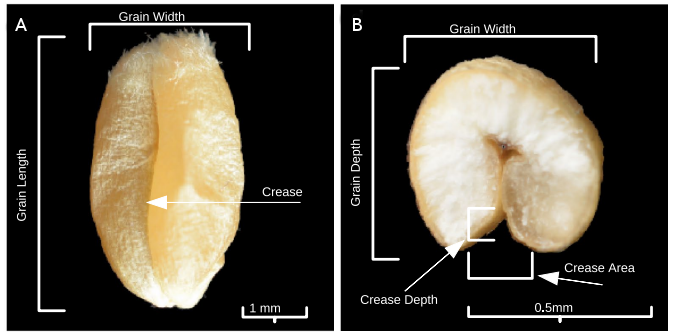
\includegraphics[width=17cm]{./images/seeds.png}
\caption{\label{fig:orga35217b}
Wheat grain labelled (\emph{left}), wheat grain cut in half (\emph{right}), adapted from Hughes et al. \cite{Hughes2017}}
\end{figure}

\section{Significance to Current Research}
\label{sec:orgb011cc7}
The biological interest in this area has been expressed in several areas of research \cite{Leigh2013}, it is proposed that the key to unlocking diversity in the wheat genus lies in these ancestor, undomesticated species \cite{Cockram2007}.

This research has the potential to be useful in several areas including: crop breeding; disease resistance; environmental stress. Each of these areas depend on making informed decisions in order to direct experiments. By producing information at an individual seed level, this study has been able to provide data that can offer suggestions of plant potential and behaviour.

Often, the most sought after traits are centred around thousand-grain-weight (TGW) as well as standard deviation of seed shapes. During harvesting, filters are used to only allow ideal shaped seeds through. This means that, potentially, despite a breed of wheat providing a high average volume of seed in reality much of it may go to waste if the shapes are not uniform. This research aims to alleviate this problem and provides low level information which is sorely required.

The individual images in figure:\ref{fig:org20e9371} show, at a glance, the diversity and also the difference in the wild and cultivated (domesticated)
species. This work allows for these differences to be quantified and evaluated into useful metrics for answering research based questions.

By better understanding the morphometric deviations in wheat species, more informed choices can be made when it comes to breeding wheat for the future and to fulfil ever-changing requirements.

\clearpage

\begin{figure}[htbp]
\centering
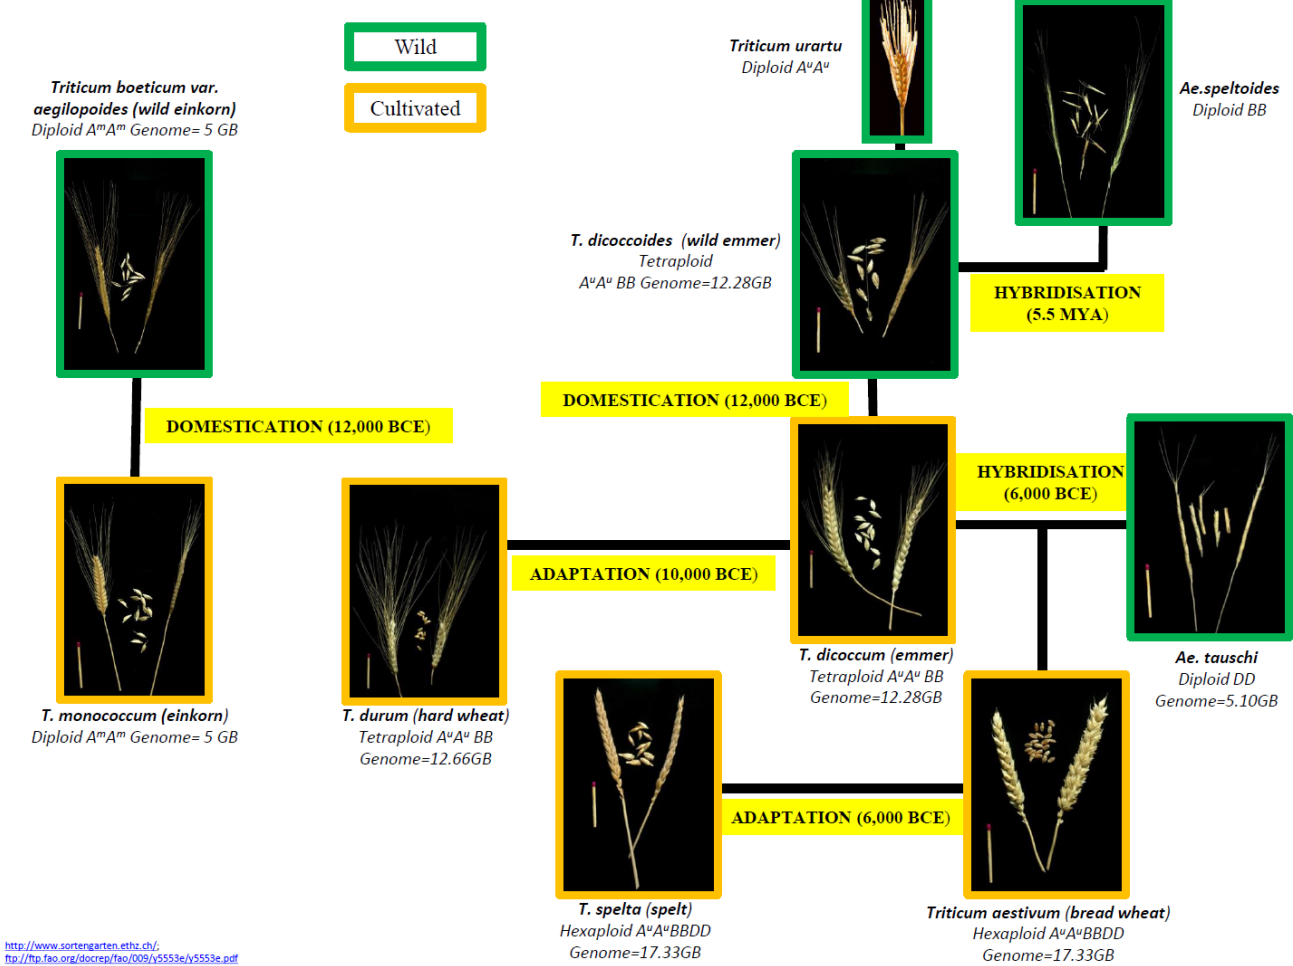
\includegraphics[width=17cm]{./images/philotree.png}
\caption{\label{fig:org20e9371}
Phylogeny of wheat genotypes (Provided by Dr. Hugo Oliveira)}
\end{figure}

\section{Aims and Objectives}
\label{sec:org9abed7e}

The overarching aim of this project has been to create several pieces of software which aid in answering the biologically significant questions outlined. As well as to prove/disprove the hypothesis stated below.

The software created is robust in order to duplicate results and is flexible as to allow for further studies to be carried out and to use the same method.

Novel additions have been made to existing image analysis libraries in order to make them more flexible for this project. Figure:\ref{fig:org2d1de68} illustrates the range of diversity

Furthermore, the library written allows for easy data organisation and automation of otherwise difficult tasks such as concatenating data from multiple sources and graphing of information. Full documentation and integrated testing allows for a suite of tools which can be built upon in future and reduce the amount of effort required for similar studies to be carried out and analysed.


\section{Hypothesis}
\label{sec:org8817fe9}
To provide a full spectrum of analysis the null-hypothesis of this work is presented as investigating if there are morphometric differences in the seeds of several wheat varieties outlined in figure:\ref{fig:org20e9371}.

The comparison pairs are as follows (where W indicates wild genotypes and D domesticated.):

\begin{enumerate}
\item \emph{T. monococcum} (2N|D) and \emph{T. beoticum} (2N|W)
\item \emph{T.dicoccum} (4N|D) and \emph{T. dicoccoides} (4N|W)
\item \emph{T. spelta} (6N|D) and \emph{T. aestivum} (6N|D)
\item \emph{T. dicoccum} (4N|D) and \emph{T. durum} (4N|D)
\item \emph{T. beoticum} (2N|W) and \emph{T. dicoccoides} (2N|W)
\end{enumerate}

These comparison groups where chosen, with help from researchers at the National Plant Phenomics Centre, based on their ploidy and also on their domestication grouping. This maximises the potential of this research by isolating features and attributes of wheat based on domestication status.
\begin{figure}[htbp]
\centering
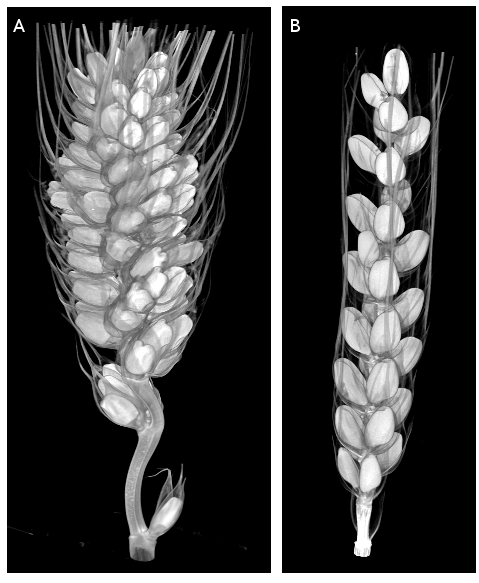
\includegraphics[width=10cm]{./images/spikes.png}
\caption{\label{fig:org2d1de68}
Scans of wheat, showing diversity in Population, Compactum (6N) left, Durum right (4N)}
\end{figure}

\section{Challenges Overview}
\label{sec:org02aa927}

The challenges which this project tackles come in two flavours: Computational and Biological. As such keen awareness of these is needed to appreciate the novelty of this work.

\subsection{Biological Challenges}
\label{sec:org3da2204}
Previous studies have been able to demonstrate that variation in wheat grain morphology can be partially explained, in 2010 Gegas et al. demonstrated this through a 99.4\% 2 component PCA \cite{Gegas2010}. However there is much left to do in terms of formal classifications and descriptions of these differences. This project deals with this problem through computational analysis.

Two effects run parallel in this study, both of these need to be accounted for in the analysis, and questions need asked in a manner to extract each effect independently:

\begin{enumerate}
\item The effects of ploidy in wheat.
\item The effects of domestication in wheat.
\end{enumerate}

Hypothesis are required to take into account, both of these effects so as not to misidentify results.

\subsection{Computational Challenges}
\label{sec:org1a51580}
Using \textmu{}-CT data in plant sciences is becoming more and more common \cite{Tracy2017,Jhala2015,Hughes2017,Metzner2015} and whilst a lot of studies focus on the traits of grains specifically no formal model has been created, no accepted data format. This is a data engineering problem and the methods described in this project address this.

Further to data organisation, proposals are made for the statistical analysis which should be used. This allows for studies to become more robust and repeatable, thus strengthening the studies overall.

The biological material used in this research is much more diverse a population than has been previously studied with \textmu{}-CT image analysis, this requires current computer vision methods to be adapted in order to be accurate.

\section{Deliverables}
\label{sec:org5112205}

This project provides three final deliveribles:

\begin{enumerate}
\item A flexible software suite written in \emph{Python} that provides a standardised method for analysing and interpreting \textmu{}-CT data output.
\item A Graphical User Interface (GUI) which offers a point and click method for data gathering, graphing and manipulating \textmu{}-CT data, using the library from deliverable 1 as a backend.
\item Answers to the proposed questions (hypothesis), the \emph{Results} and \emph{Discussion} sections of this report provides this.
\end{enumerate}

\chapter{Software Design, Implementation and Testing}
\label{sec:orgabc4bdf}
This chapter outlines choices and methodologies employed in the software engineering aspect of this project, as well as highlighting the key functional requirements and implementation decisions.

\section{Functional Requirements}
\label{sec:org0e4b32a}
Requirements for this project are split between software requirements for both the CT Analysing Library and the CT GUI Application and the research requirements (i.e. the answers to the proposed hypothesis). Here the requirements for the software are discussed:
\subsection{Requirements for CT Analysing Library}
\label{sec:org46a9460}

These are the functional requirements for the Python library produced:

\begin{multicols}{2}

  \begin{enumerate}
  \setcounter{enumi}{-1}
  \item Provide an OOP means to deal with data
  \item Make gathering of data simplified
  \item Handle Saving of data in a useable format
  \item Easily enable data transformations
  \item Perform hypothesis testing
  \end{enumerate}

  \columnbreak

  \begin{enumerate}
  \setcounter{enumi}{4}
  \item Process rejoining of split scans
  \item Handle Removing of erroneous data
  \item Enable matching data to external information
  \item Auto plot data (boxplots, histograms etc.)
  \item Allow easy filtering of data
  \end{enumerate}

  \columnbreak

\end{multicols}

\subsection{Requirements for CT GUI Application}
\label{sec:org4020bac}

\begin{multicols}{2}

  \begin{enumerate}
  \setcounter{enumi}{9}
  \item Provide a intuitive user interface for working with CT data
  \item Allow a interaction with data without the need for programming
  \item Implement the Matplotlib plotting utility
  \item Easily join experiment data with CT data
  \item Use an MVC model
  \end{enumerate}

  \columnbreak

  \begin{enumerate}
  \setcounter{enumi}{14}
  \item Implement the CT Analysis Library
  \item Display data visually
  \item Dynamically create graphs
  \item Provide hypothesis testing
  \end{enumerate}

  \columnbreak

\end{multicols}

\section{Software Development Methodology}
\label{sec:org4c43478}
This project made use of formal design methods and strict organisation whilst being flexible to change. Overall the design took a hybridised form in order to best suit the scientific environment which this domain specific software is built for.

Data analysis drove the direction of the project, as a result an agile methodology was adopted.
Weekly sprints were implemented as a list of "todo's", these were written on a Monday morning based off of the previous week's list.

Critical self-evaluation was performed by means of a "one-man SCRUM" meeting, this is a technique which requires self-discipline in order to accurately find faults and areas for improvement \cite{Andrews}.

Further to this, regular meetings with research staff, at the National Plant Phenomics Centre,  allowed for a developer-client relationship which SCRUM defines as being key. During these meetings details of the research was discussed and ideas given as to how future experiments could proceed. This allowed for critical decisions to be made as to software design and overall structure.
\section{Sprint Timeline}
\label{sec:org02d8c6a}
The implementation of this work was done following agile sprint planning, treating each week as a encapsulated working frame, for each of these a detailed organisational programme was created, discussed with supervisors and then used to formulate plans of action for following up on.

\subsection{Sprint - Week 0}
\label{sec:org575ecb3}
Initial planning was taken out, discussions with researchers at the National Plant Phenomics Centre (NPPC), to create a general set of targets and research goals.

A website was built in order to host weekly progress reports, this was used to share with supervisors and with staff at the NPPC. It also provided a list of discussion points to go through at weekly meetings.

A bug was identified in image analysis software, this was raised to be fixed a later date.

A literature review was taken out to highlight the novelty of this research, as well as current trends in the field in terms of analysis and known/accepted information.

\subsection{Sprint - Week 1}
\label{sec:orgbd2baa1}

Initial running of grain analysis software was performed multiple times, as per instructions in literature \cite{Hughes2017}, multiple parameters for minimum and maximum expected sizes of grains needed to be tested. Data which was produced was very noisy and would require further work.

Spike work was carried out in investigating the potential of using a skeletonising method on the wheat spikes. The hope behind this was to simplify structure in a three dimensional structure, of 1 pixel thick lines. This technique is often used in plant root analysis \cite{Mairhofer2015,Daly2017}. Experimentation with these methods were technically challenging and a decision was made to revisit if time permitted at the end of the project.

A key function of the CT Analysis Library was created, showing in listing:\ref{orge75c7bc}. The method enables additional experiment information to be joined with extracted seed data. This provides a way of grouping seeds into more useful groupings than just their scanning data.

An issue was identified in the choices of testing which are typically used in these studies, the use of ANOVA and Student's T-Test, for example, are best used with parametric data, that is to say data where distribution is normally distributed. Further reading into this presented the use of Box Cox transforms as a method to counter these issues.

An issue was raised; a method for visualising outliers in the data could provide greatly beneficial insight into finding errors. If time was available at the end of the project, this would be explored further.

\subsection{Sprint - Week 2}
\label{sec:org2ab6120}

Spikes of wheat are scanned in two separate imaging cycles sometimes, this is because the tube used by the \textmu{}-CT machine are 10cm tall and often a spike will exceed this. In order for full analysis to be carried out these separate scans need to be rejoined. A method for doing this was added to the python Analysis Library.

An initial Model-View-Controller (MVC) model was constructed for how a GUI might take form around. Using this several wire-frames were created

An idea for how data could be cleaned was created by using the information found in previous studies \cite{Hughes2017}. From this reported data minimum and maximum expected size could be assumed for wheat grains in terms of volume.

Decisions to move the CT Grain Analysing Library towards an object orientated model were made during this sprint, after evaluating the potential of a functionally programmed model or a object one. Handling everything in terms of classes was decidedly easier in terms of understanding how to use the library.

\subsection{Sprint - Week 3}
\label{sec:orgfc6a7cb}

A lot of progress was made on constructing a GUI here, dynamic plotting was put together as a proof of this concept. Histograms of the data were able to be made by using the mouse to select which attribute to measure.

GUI elements such as navigation, data tabs and file menus were added to make more clear to the user how functionality should work.

A novel and new method for generating documentation was created specifically for documenting this software library. Using a plain text format, doc strings from python code was used to make a single easy to read PDF to be distributed with the software package.

Another piece of functionality was introduced to the GUI that would enable the user to view the data they had loaded as a single 2 dimensional data frame. This is for quickly viewing data as a single source and all together. This had arisen as a functionality desired by researchers in a previous weeks meeting.

\subsection{Sprint - Week 4}
\label{sec:orga12f38d}
A new method for watershedding was developed and deployed in the data extraction pipeline, this moved towards using euclidean distance transforms. Allowing for the more complex shapes which this data set presented as a problem to be fully and properly segmented.

Further work was done in terms of the GUI to enable matplotlib and seaborn library integration with the dynamic plotting features which were developed previously.

Custom exceptions were written for the CT Analysing Library, these exceptions allow for more detailed feedback to a programmer when they perform actions which might result in erroneous data processing. In particular a "NoDataFoundException" was made for when empty data files where found in searching.

Current versions of doc strings were enhanced to match with newer functionality which had been added in recent weeks, and documentation was regenerated.

\subsection{Sprint - Week 5}
\label{sec:orge56dbc0}
Functions were added to the CT Analysing Library which would allow for aggregation of data columns, this meant that averaging functions could be performed on a per-spike basis. Mean, standard deviation, sum and count functions were applied by default.

Further research was carried out into data transforms which are commonly used in data science; Principal component analysis, linear modelling and multivariate analysis were topics researched as possibilities for inclusion in this library.

\subsection{Sprint - Week 6}
\label{sec:org39fb04c}
Preparation for a mid-project demo took up the majority of this sprint, ensuring data which had been gathered to date was well understood was vital.

A presentation was created using data extracted via the CT Analysing Library, this was in the mode of figures and graphs which could then be used to better explain the theme of the project.

\subsection{Sprint - Week 7}
\label{sec:org9cbb46a}
An initial implementation of principal component analysis was tested and found to be useful, a considerable amount of time was dedicated to refactoring the code-base to allow for new data transforms to be easily incorporated.

Additions to the graphing section of the library also allowed for splitting data into multiple plots which could then be featured side-by-side, separation of data helped contribute to seeing the differences in the data.

Some initial ideas for unit testing were written up, an investigation into which platform and library were best to use was carried out. This had to be taken into consideration as testing a GUI required some additional software to simulate a user testing widgets and onscreen objects.

\subsection{Sprint - Week 8}
\label{sec:orgc5aca3b}
With data extraction parameters finalised, a new watershedding method implemented and a more robust selection process implemented the data was now fit for hypothesis to be tested.

Through meetings with researching staff, the five key hypothesis/null-hypothesis had been formed and the grouping of the data well defined. This allowed for initial Null-Hypothesis-Significance-Testing (NHST) to be carried out. The initial results found were not representative of the data. A requirement for new hypothesis testing was now required.

The \emph{PyTest} library was decided upon, this was used as a unit testing framework for both the Analysis Library and the GUI software. In total around 50 tests were devised.

\subsection{Sprint - Week 9}
\label{sec:org738606b}
More graphing options were added to the GUI, these came from the boxplot functionality which the updated CT Analysing Library made available. A new type of grouping by sub-type was added. This let multiple plots be displayed for the same feature i.e. viewing a histogram of volume but split by genotype. This new feature required a rework of the dynamic plotting functionality. This refactoring took a considerable amount of time and work.

An initial solution to hypothesis testing was added in the form of Welch and Student T-Tests to first the CT Analysing Library and then to the GUI also. The GUI now had an additional tab added specifically for testing groups of data.

\subsection{Sprint - Week 10}
\label{sec:org721fd78}

A previous issue was highlighted in meetings of the data being ill-suited to normally accepted statistical testing and NHST in general. Through research a new method was devised that was able to use Bayesian statistics to carry out hypothesis testing \cite{Kruschke2012}. This new method of hypothesis testing was added into the CT Analysing Library, requiring a lot of work in data transforming and preparation in order for correct, robust and repeatable model fitting to be carried out.
Previous research questions were repeated, using this method. This time new and significant findings were uncovered.

\subsection{Sprint - Week 11}
\label{sec:orgc645ec5}
A feature freeze was enforced during the 11th week of the project. This was to ensure time was allocated for completing work, finalising unit tests and documentation. The > 50 unit tests were finalised, completed and ensured to be passing. Documentation was completed and exported.

\section{Language Choices}
\label{sec:org310608b}
Both the CT Analysing Library and the CT Analysing GUI are implemented using the Python programming language, it has been developed and tested in versions 3.5 and 3.6 (Python 2 is not supported at all by this project).

In scientific programming three of the most commonly used languages are Python, R and MATLAB \cite{Ozgur2016}.

These three languages are able to provide all the features which this project requires. However Python was chosen for several reasons.

MATLAB could not be used as a potential language due to it being pay to use software, as this project aims to be accessible, the cost of software would greatly reduce the scope of access.

R is a valid candidate, it provides all of the statistical capabilities required by the project, it also provides packages for creating GUI based applications, it is fast and it is widely used in scientific computing and data science.

The main deciding factor is Python's wealth of resources, adoption rate and the developer of this project being vastly more experienced with Python's ecosystem than R's.

\section{Designing Process}
\label{sec:orgbdd298a}
Through meetings and emails, the agile principles of communication over comprehensive documentation was used. Where conversations were decidedly much more beneficial than complex planing prior to developing a product.

Graphical elements, such as the graphing functionality of the CT Analysing Library and the CT GUI Application were sketched using wire-frames whilst in meetings where the potential users (clients) could provide their ideas.

In figure:\ref{fig:org331bd84} an example of the wire-frames created during meetings is show (A), next to it is displayed the final look of the loading window (B).
\begin{figure}[htbp]
\centering
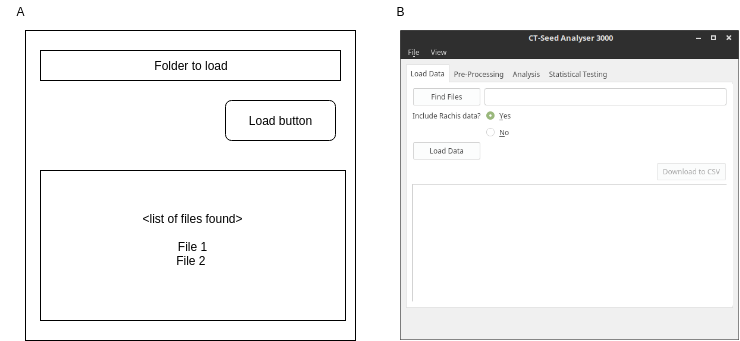
\includegraphics[width=16cm]{./images/wireframe1.png}
\caption{\label{fig:org331bd84}
Wire-frame of the GUI loading data window}
\end{figure}

Similarly, figure:\ref{fig:orge5315a8} provides the initial wire-frame (A) of how the analysis window could have looked and what kind of GUI elements would be required, again, next to it is the final analysis window (B)
\begin{figure}[htbp]
\centering
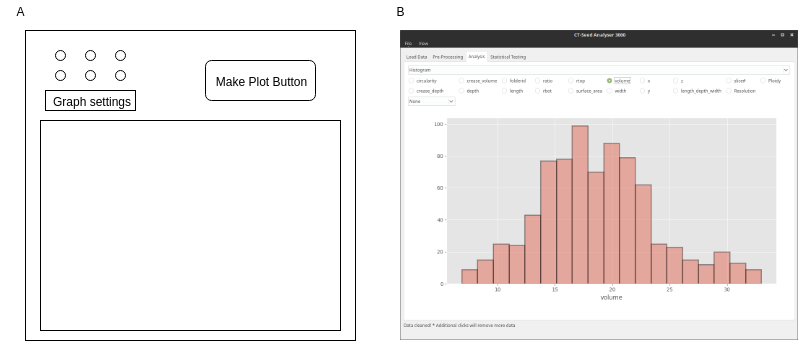
\includegraphics[width=16cm]{./images/wireframe2.png}
\caption{\label{fig:orge5315a8}
Wire-frame of the GUI analysis window}
\end{figure}
\section{Documentation}
\label{sec:orga200a75}
Whilst an agile approach was used, some documentation was created for use with the CT Analysing Library.

The provided CT Analysing Library comes with "human-readable" format. Where most documentation generators (Doxygen, Pydocs, Javadocs etc.) implement very well structured and comprehensive documentation, the output is generally not very friendly and easy to read. Particularly for non-career-programmers. A core feature of these provided software implementations are that they are well suited for a biologist, researcher or statistician to use.

This documentation generator was purpose created, implemented in LISP and provided in listing:\ref{org1db3016}.

Beyond this, inline commenting is provided for supplied software. Keeping in line with the agile development ethos the software is self-documented and self-evident. A brief example of this is shown in listing:\ref{org52bea07}

Documentation for the CT GUI application is provided as a visual user guide, and provides sample data for the user to test with.
\section{Software Library Choices}
\label{sec:orgb244413}
The software libraries used for this project focus around data manipulation, where possible core libraries of the Python language were used and only well supported, established and documented libraries were chosen. Software support is a major requirement for reproducible results.

All software packages used in the Analysing Library are required by the CT Analysing GUI as the Library is a dependency of it. The GUI has a single separate requirement \emph{PyQT5}.
Table:\ref{tab:orgd79dfdb} contains a full listing of all software used and required by this project.
\subsection{Numpy}
\label{sec:org720e52a}
The Numpy library is one of the most commonly used additions to the Python ecosystem, it is fundamental to many data science projects. Here it is used to handle data lists, arrays and structures. There is no viable alternative to this package and it is required by Scipy and Statsmodels.
\subsection{Matplotlib/Seaborn}
\label{sec:orge76c177}
Matplotlib acts as the plotting backend for the project. The Seaborn package acts as a porcelain for matplotlib and makes graph creation and decoration much easier.
\subsection{Scipy}
\label{sec:org46fd6cf}
Data transforms such as Box Cox and PCA are dependant on the functions of the Scipy library. Alternatives are available, however this is the most well established and often used library for these functions.
\subsection{Pandas}
\label{sec:org9a134f8}
Pandas is used to read the CSV files which the raw data is stored in. This library converts and stores data in dataframes which are used throughout this project to manipulate data.
\subsection{Xlrd}
\label{sec:org311ee71}
This extension library is required in order to read Microsoft encoded files. Extra experiment information can be provided with the "xlsx" extension.
\subsection{Statsmodels}
\label{sec:orgeb40276}
Bayesian hypothesis testing is provided through this library.
\subsection{PyQT5}
\label{sec:orga60edbc}
There were many options for creating a user interface in Python, the language provides its own core library via the \emph{TKinter} module. However PyQT is a port of the QT framework, one of the most widely used libraries for GUIs in software development. It is cross platform, robust and has excellent documentation and user-guides.
\section{Version control}
\label{sec:orgbc709d7}
This project has used Git version 2.7.4 throughout. The structure of the project has been as submodules of a larger project.

By using submodules the CT Grain Analysing Library could be kept in sync with the GUI aspect of the project.

Additionally, \emph{setup.py} has been used to provide installation of the library, the code for this can be seen in listing:\ref{org6334f9d}. Using \emph{setup.py} provides a quick and easy way for any user to install the software, along with any dependencies.

\subsubsection{Issue Tracking}
\label{sec:orgcd5c6ad}
Issues were tracked during the project, both in personal notes and in the Git interface as illustrated in figure:\ref{fig:org91fc80c}
\begin{figure}[htbp]
\centering
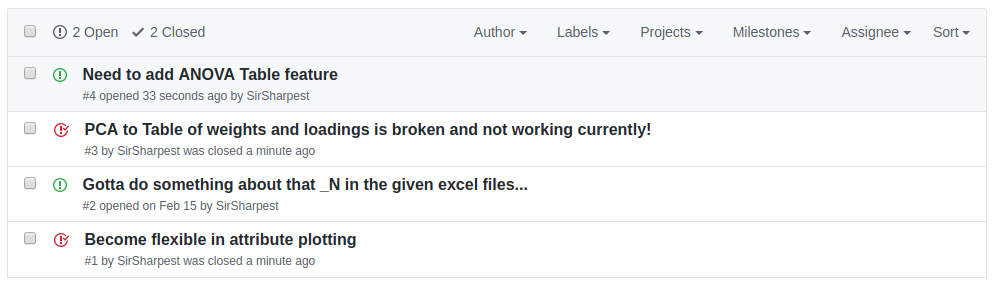
\includegraphics[width=12cm]{./images/github.png}
\caption{\label{fig:org91fc80c}
Github Issue Tracking}
\end{figure}

\section{Implementation}
\label{sec:orgb8852a6}
Strict software engineering principles were applied during creation of this project. The use of standards, design patterns and code-linters have been used throughout to minimise the possibility of errors and to create wholly extendable software. These devices enable understandable and self-documented code allowing future users to quickly start using the provided packages.
\subsection{Standards}
\label{sec:org3f1cc27}
The main standard adhered to for software provided by this project is the PEP8 style guide \cite{VanRossum}. The principle behind this coding style, as stated by Guido van Rossum, is "Code is read much more often than it is written". This makes this styling guide perfect for the chosen agile methodology of self-evident documentation in the software.

In addition to PEP8, a Python code linter Flake8 has been used to prevent "code smells", bad formatting, incorrect white space usage etc.

\subsection{CT Analysing Library Design Pattern}
\label{sec:org60277c7}
The CT Analysing Library uses a Singleton style design pattern. A single data object is created from a \emph{CTData} class.

A very functional paradigm is used by this library. By applying mapping and filter style functions data elements can be passed to the supporting modules: \emph{data\_transforms.py}; \emph{graphing.py}, \emph{statistical\_tests.py}. These modules enable scientific functions to be applied to the \emph{CTData} object. A UML style class diagram is shown in figure:\ref{fig:orged21911}, here the interactions of the classes can be seen, as well as their internal functions.

\begin{figure}[htbp]
\centering
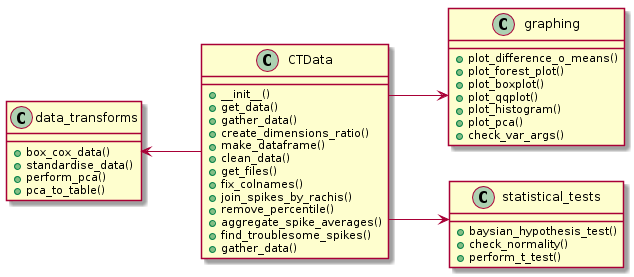
\includegraphics[width=12cm]{./images/ctdata.png}
\caption{\label{fig:orged21911}
CT Analysing Library UML}
\end{figure}

\subsection{CT GUI Application Design Pattern}
\label{sec:org5582c03}
The Model-View-Controller (MVC) design pattern is one of the most commonly structures for creating user interfaces. It allows for the user's view/interface code to be separated from the model, the code which changes the data. The model and the view communicate and update each other via the controller element of the design.

The QT framework provides "connectors" which act as triggers/activations for functions, these are set off by the user providing either keyboard or mouse based input.

\begin{figure}[htbp]
\centering
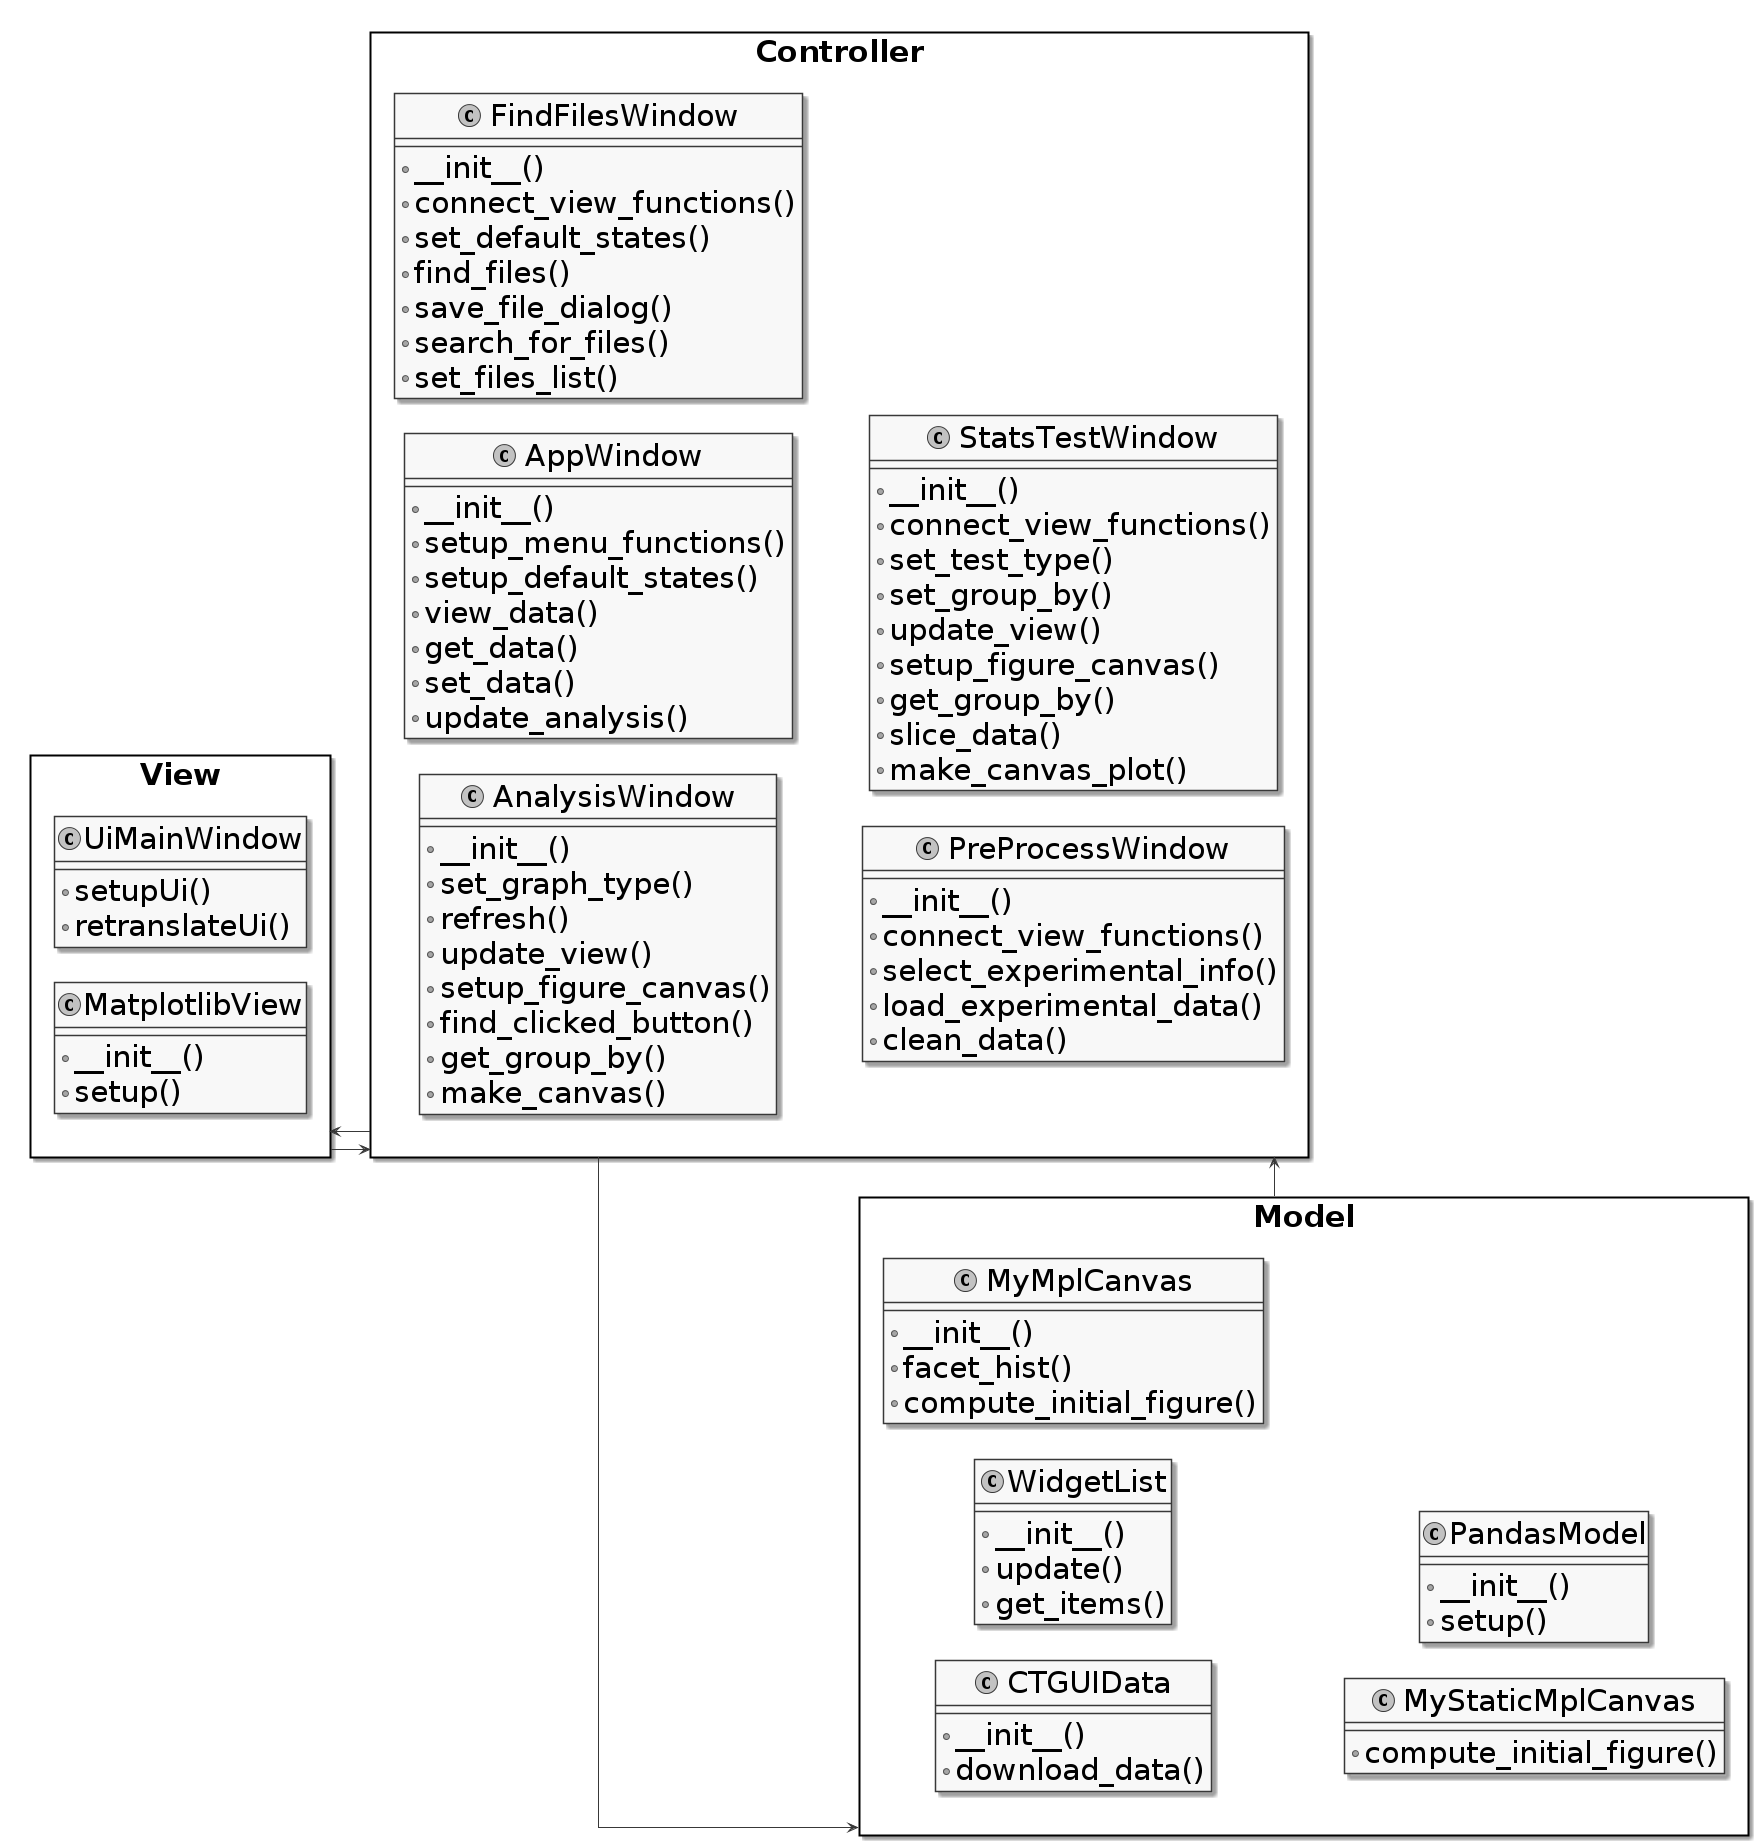
\includegraphics[width=15.2cm]{./images/ctgui.png}
\caption{\label{fig:orgf5eb2c4}
CT Analysing GUI UML}
\end{figure}
\section{Library Versioning}
\label{sec:orge09ab6b}
The development of this project was performed using the Python \emph{virtualenv}. This is a virtual environment package which Python offers, it allows for an isolated working copy of the project.

By developing in this manner, libraries were ensured to be using the correct versions required by the software.
 \clearpage
\section{Testing}
\label{sec:org6a41fad}
Testing was performed both in acceptance testing by using user feedback, the functional requirements and the ability to use the software to answer the hypothesis of the research elements of this project. Further to this, unit testing was performed to allow for automated testing as well as test-driven-development of features.
\subsection{Feedback Forms}
\label{sec:org76bccd3}
Feedback and constructive suggestions were made by researchers at the National Plant Phenomics Centre, these were submitted via the Google forms service.

These provided a method of acceptance testing by those who would be using the software to help with investigating data. Page 1 of the given form is shown in figure:\ref{fig:org68c2026}. This form was completed by 3 researchers at the National Plant Phenomics Centre, feedback was very positive overall.
\begin{figure}[htbp]
\centering
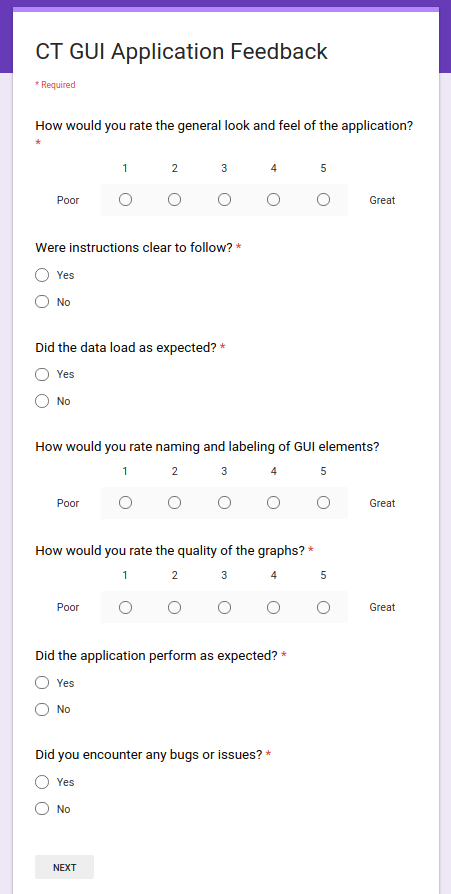
\includegraphics[width=7.3cm]{./images/feedbackform.png}
\caption{\label{fig:org68c2026}
CT Feedback form}
\end{figure}

\clearpage

\subsection{Unit Testing CT Analysing Library}
\label{sec:org3c8d830}
The unit tests for the CT Analysing Library were straightforward, using the \emph{PyTest} framework and a subset of data from a data set, these tests assert that features are implemented correctly and that the correct results are given.


\begin{table}[htbp]
\caption{\label{tab:org4552642}
Output of \emph{pytest} Unit Tests and results for CT Analysing Library}
\centering
\begin{tabularx}{\textwidth}{|l|l|X|}
\hline
I.D. & \textbf{Result} & \textbf{Test}\\
\hline
0 & \color{ForestGreen}Passed & CTData.py::test\_aggregate\_spike\_averages\\
\hline
1 & \color{ForestGreen}Passed & CTData.py::test\_clean\_data\_maximum\_removed\\
\hline
2 & \color{ForestGreen}Passed & CTData.py::test\_clean\_data\_minimum\_removed\\
\hline
3 & \color{ForestGreen}Passed & CTData.py::test\_load\_additional\_data\\
\hline
4 & \color{ForestGreen}Passed & CTData.py::test\_load\_additional\_data\_no\_data\\
\hline
5 & \color{ForestGreen}Passed & CTData.py::test\_load\_data\\
\hline
6 & \color{ForestGreen}Passed & CTData.py::test\_NoDataFoundException\\
\hline
7 & \color{ForestGreen}Passed & Data\_transforms.py::test\_box\_cox\_data\\
\hline
8 & \color{ForestGreen}Passed & Data\_transforms.py::test\_pca\_to\_table\\
\hline
9 & \color{ForestGreen}Passed & Data\_transforms.py::test\_perform\_pca\\
\hline
10 & \color{ForestGreen}Passed & Data\_transforms.py::test\_standardise\_data\\
\hline
11 & \color{ForestGreen}Passed & Graphing.py::test\_plot\_boxplot\_as\_dataframe\\
\hline
12 & \color{ForestGreen}Passed & Graphing.py::test\_plot\_boxplot\_as\_object\\
\hline
13 & \color{ForestGreen}Passed & Graphing.py::test\_plot\_difference\_of\_means\\
\hline
14 & \color{ForestGreen}Passed & Graphing.py::test\_plot\_histogram\_as\_dataframe\\
\hline
15 & \color{ForestGreen}Passed & Graphing.py::test\_plot\_histogram\_as\_object\\
\hline
16 & \color{ForestGreen}Passed & Graphing.py::test\_plot\_pca\\
\hline
17 & \color{ForestGreen}Passed & Graphing.py::test\_plot\_qqplot\\
\hline
18 & \color{ForestGreen}Passed & Statistical\_tests.py::test\_baysian\_hypothesis\_test\\
\hline
19 & \color{ForestGreen}Passed & Statistical\_tests.py::test\_t\_test\\
\hline
20 & \color{ForestGreen}Passed & Statistical\_tests.py::test\_test\_normality\\
\hline
\end{tabularx}
\end{table}


\clearpage

\subsection{Unit Testing CT GUI Application}
\label{sec:orgacc58e0}

The unit testing used for the CT GUI Application was more sophisticated than that of the Library. This testing required visual confirmation that figures and graphs generated were displayed correctly and that they showed what the user would expect, given the data.

To do this a \emph{PyTest} plugin was used, \emph{QtBot} which provides simulated user input. This allows for the GUI to be thoroughly tested, automatically.

In table:\ref{tab:org26e75de} the results of the automated testing is given along side an image of several of the tests, tests of the same graphs but with different parameters were also generated and manually verified and provided as supplemental data.

\begin{longtable}{|l|l|p{4.4cm}|C|}
\caption{\label{tab:org26e75de}
Output of \emph{pytest} Unit Tests and results for CT GUI Application}
\\
\hline
I.D. & \textbf{Result} & \textbf{Test} & \textbf{Image}\\
\hline
\endfirsthead
\multicolumn{4}{l}{Continued from previous page} \\
\hline

I.D. & \textbf{Result} & \textbf{Test} & \textbf{Image} \\

\hline
\endhead
\hline\multicolumn{4}{r}{Continued on next page} \\
\endfoot
\endlastfoot
\hline
21 & \color{ForestGreen}Passed & analysis.py:: box\_groupby\_1\_rb\_1 & \begin{center}
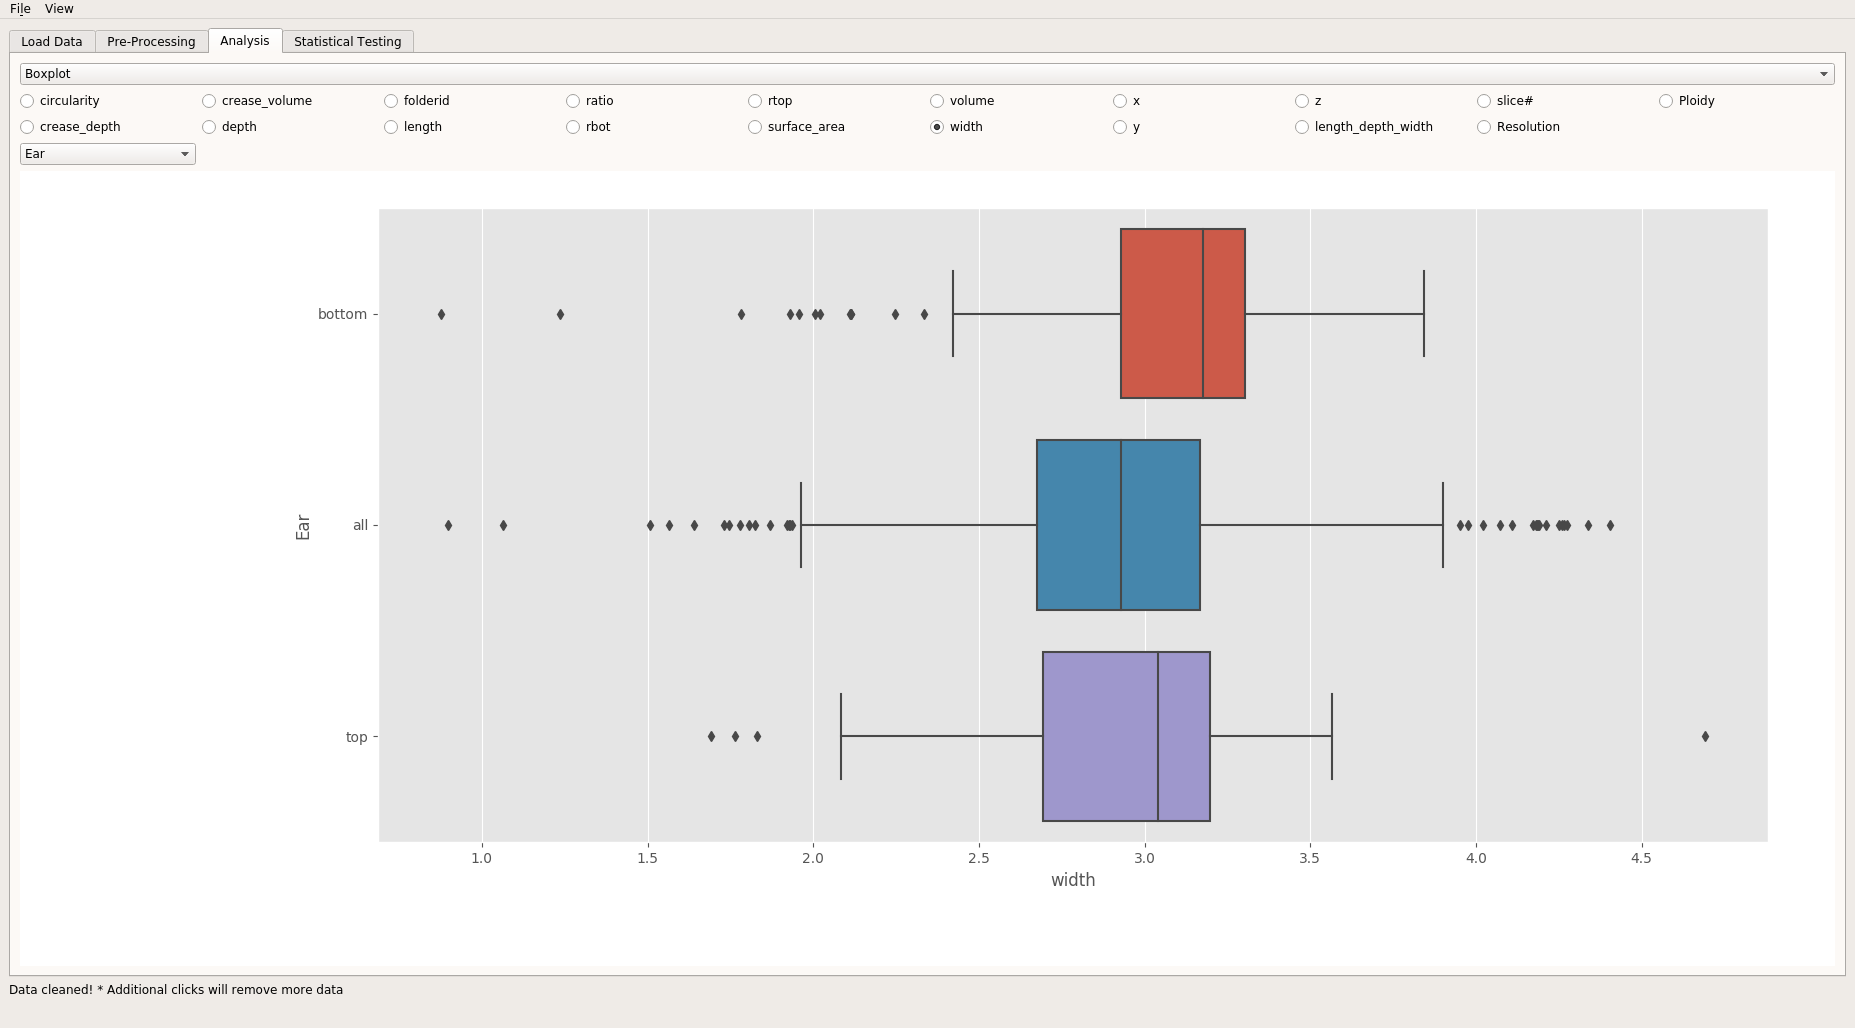
\includegraphics[width=.9\linewidth]{./images/Screenshots/analysis_window_box_groupby_1_rb_1.png}
\end{center}\\
\hline
22 & \color{ForestGreen}Passed & analysis.py:: box\_groupby\_2\_rb\_2 & \begin{center}
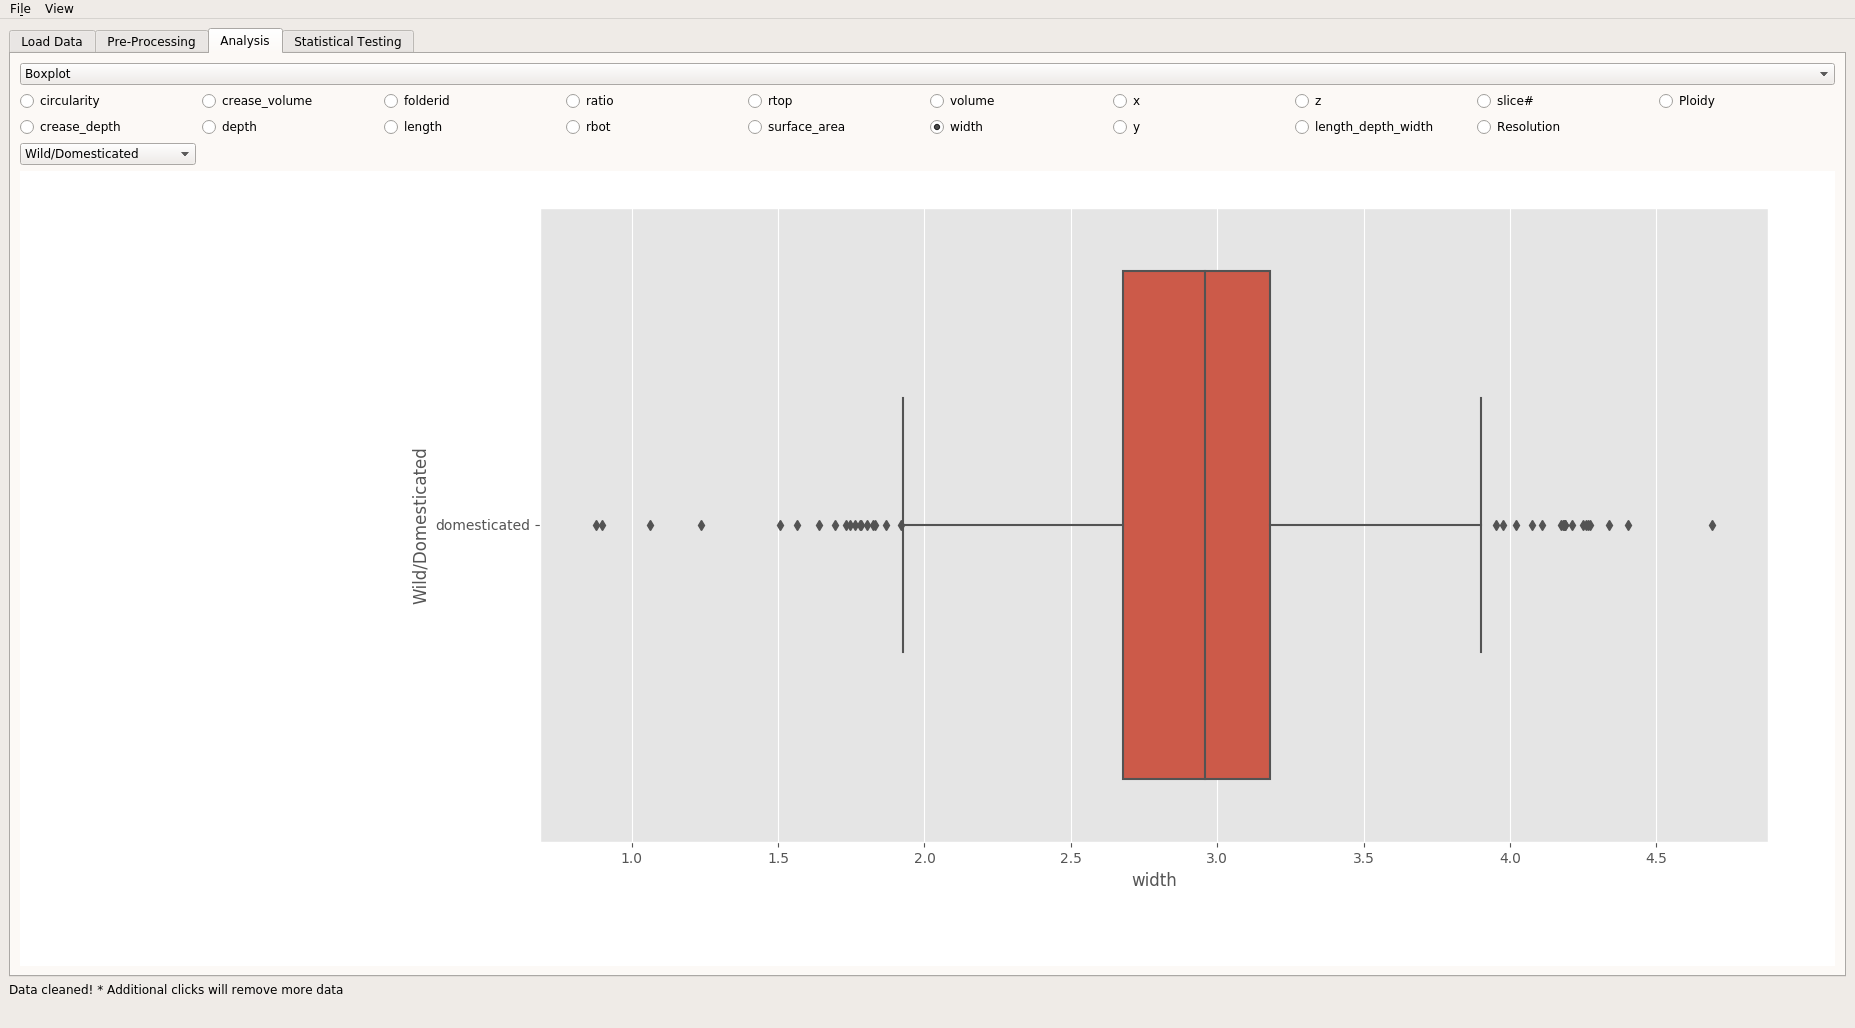
\includegraphics[width=.9\linewidth]{./images/Screenshots/analysis_window_box_groupby_2_rb_2.png}
\end{center}\\
\hline
23 & \color{ForestGreen}Passed & analysis.py:: box\_rb\_1 & \begin{center}
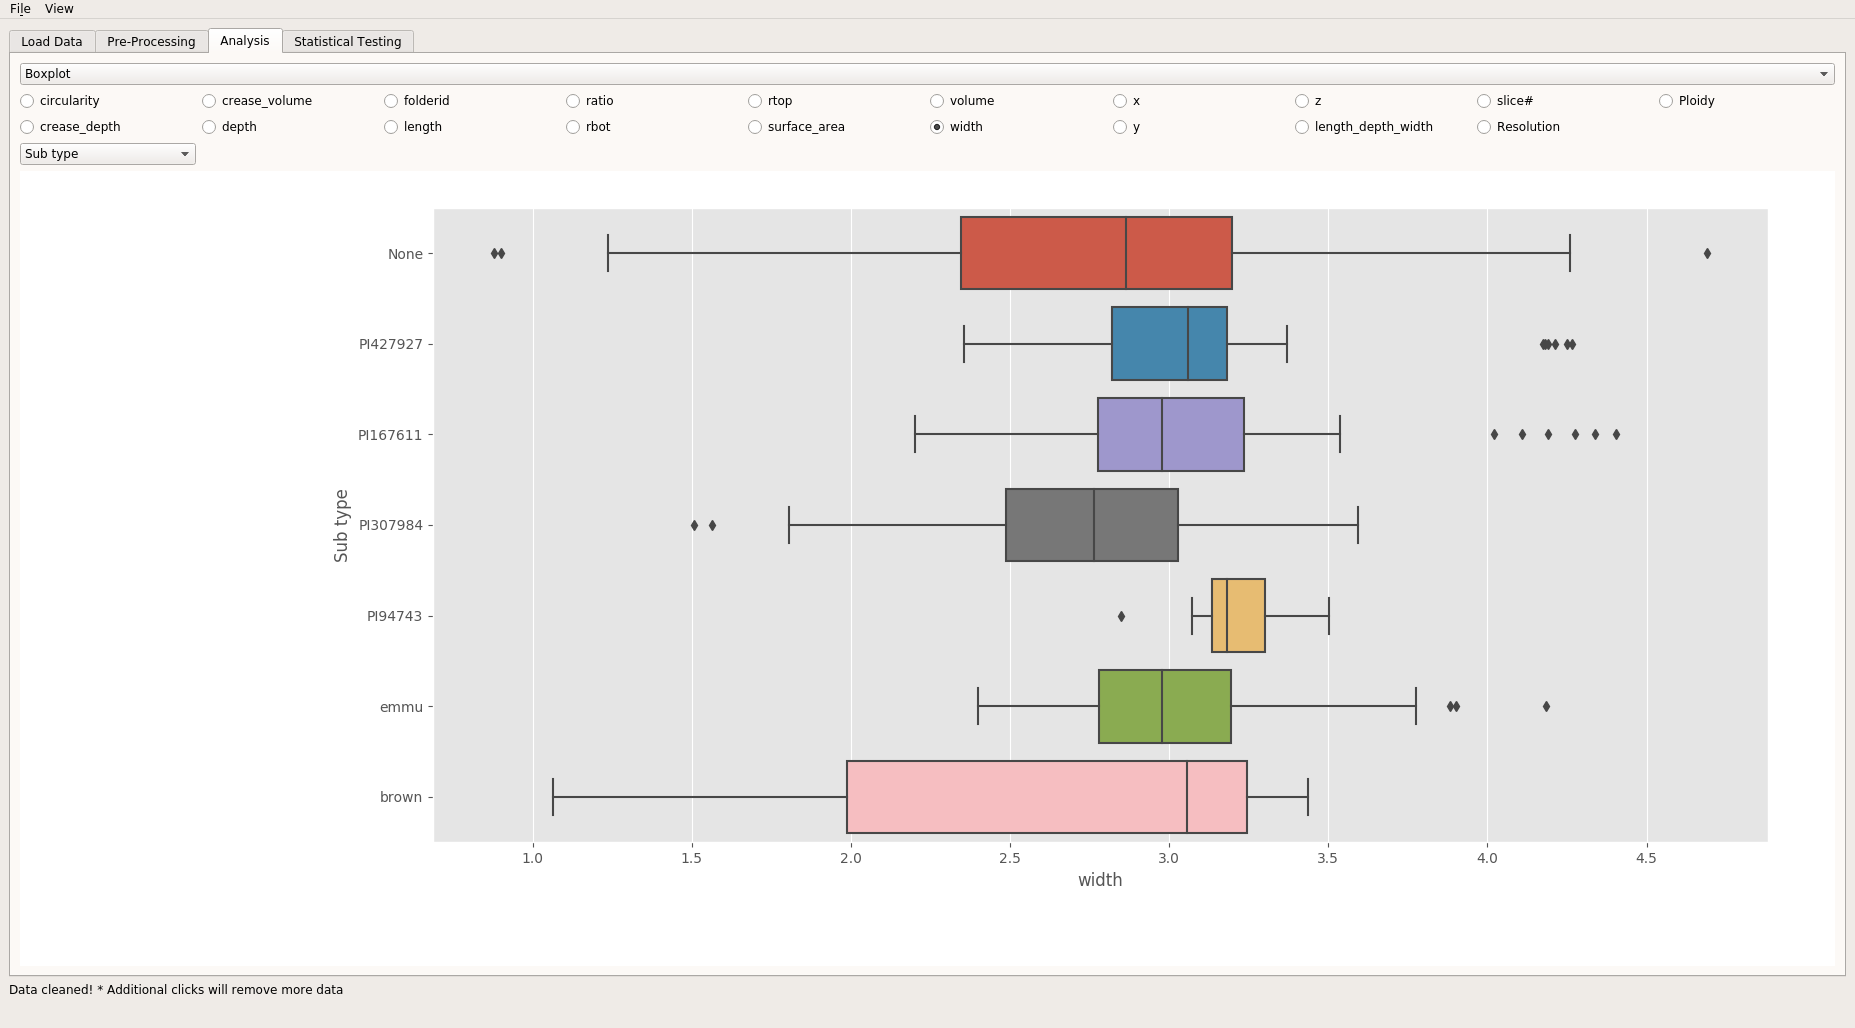
\includegraphics[width=.9\linewidth]{./images/Screenshots/analysis_window_box_rb_1.png}
\end{center}\\
\hline
24 & \color{ForestGreen}Passed & analysis.py:: hist\_groupby\_1\_rb\_1 & \begin{center}
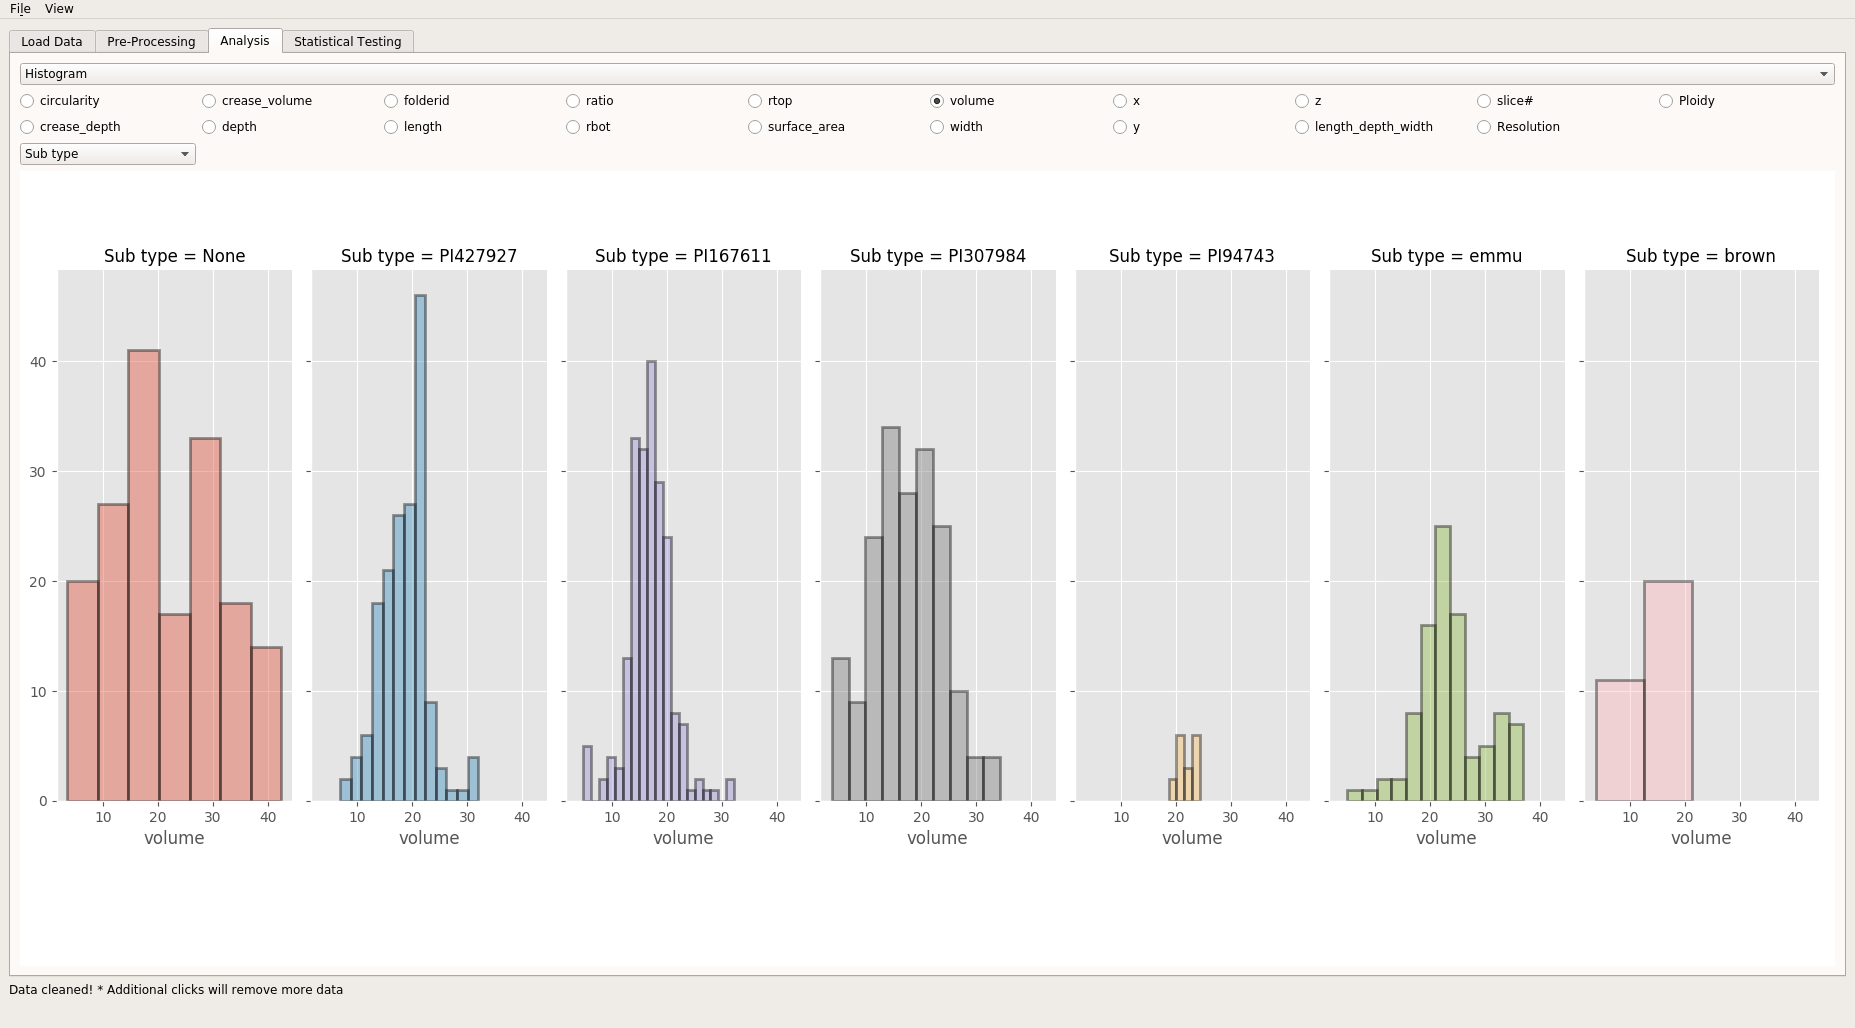
\includegraphics[width=.9\linewidth]{./images/Screenshots/analysis_window_hist_groupby_1_rb_1.png}
\end{center}\\
\hline
25 & \color{ForestGreen}Passed & analysis.py:: hist\_rb\_1 & \begin{center}
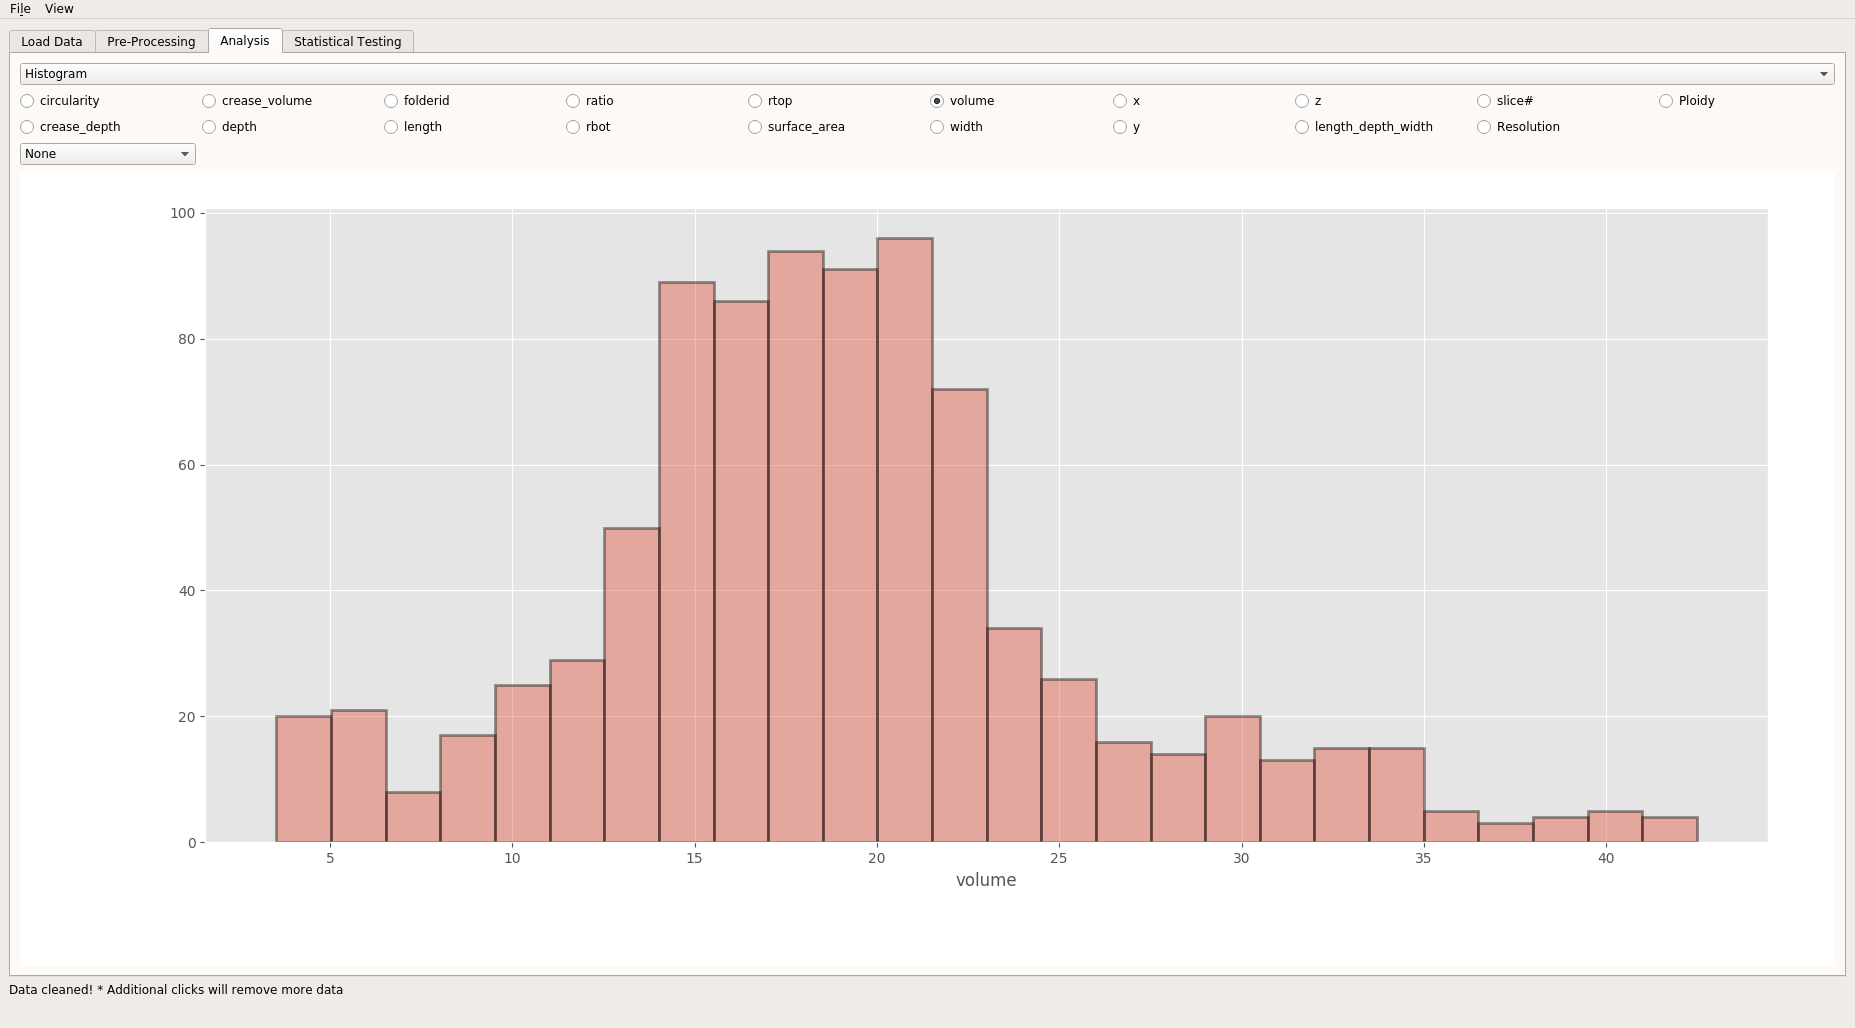
\includegraphics[width=.9\linewidth]{./images/Screenshots/analysis_window_hist_rb_1.png}
\end{center}\\
\hline
26 & \color{ForestGreen}Passed & hypothesis\_tests.py:: bayesg1\_att\_1 & \begin{center}
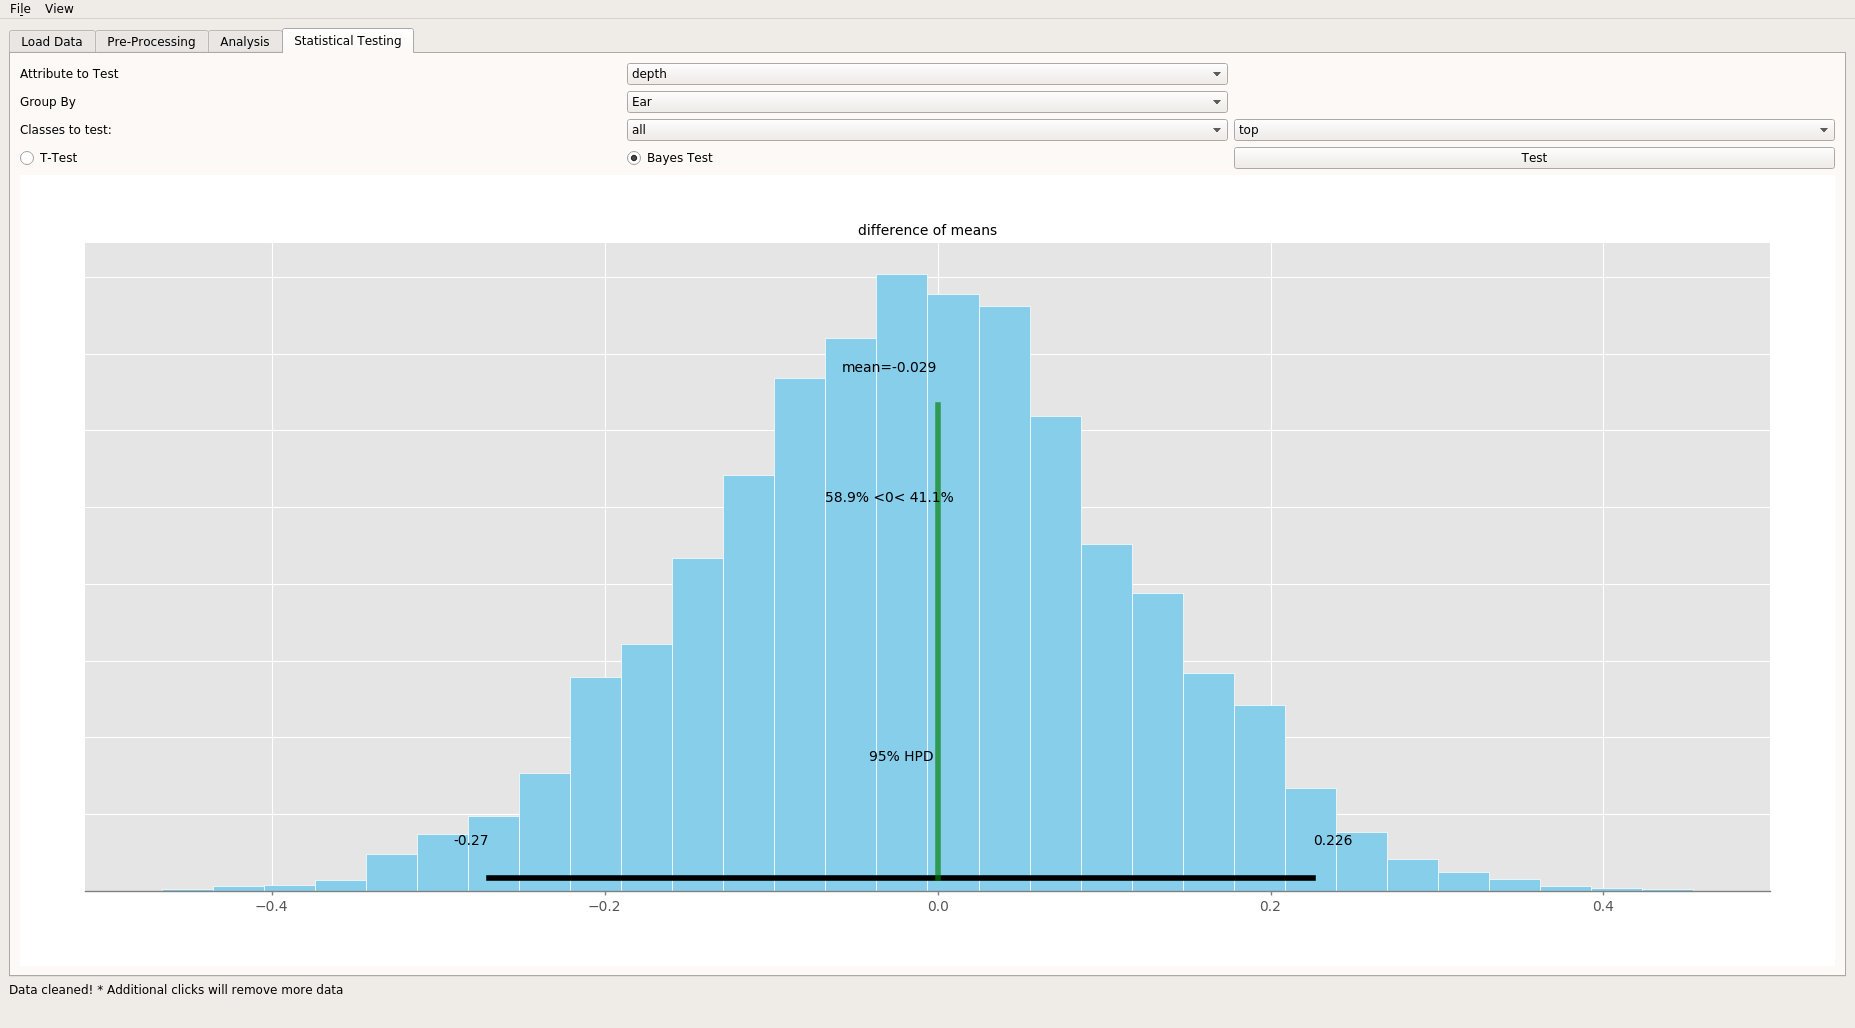
\includegraphics[width=.9\linewidth]{./images/Screenshots/hypothesis_bayestest_g1_att_1.png}
\end{center}\\
\hline
27 & \color{ForestGreen}Passed & hypothesis\_tests.py:: tg1\_att\_1 & \begin{center}
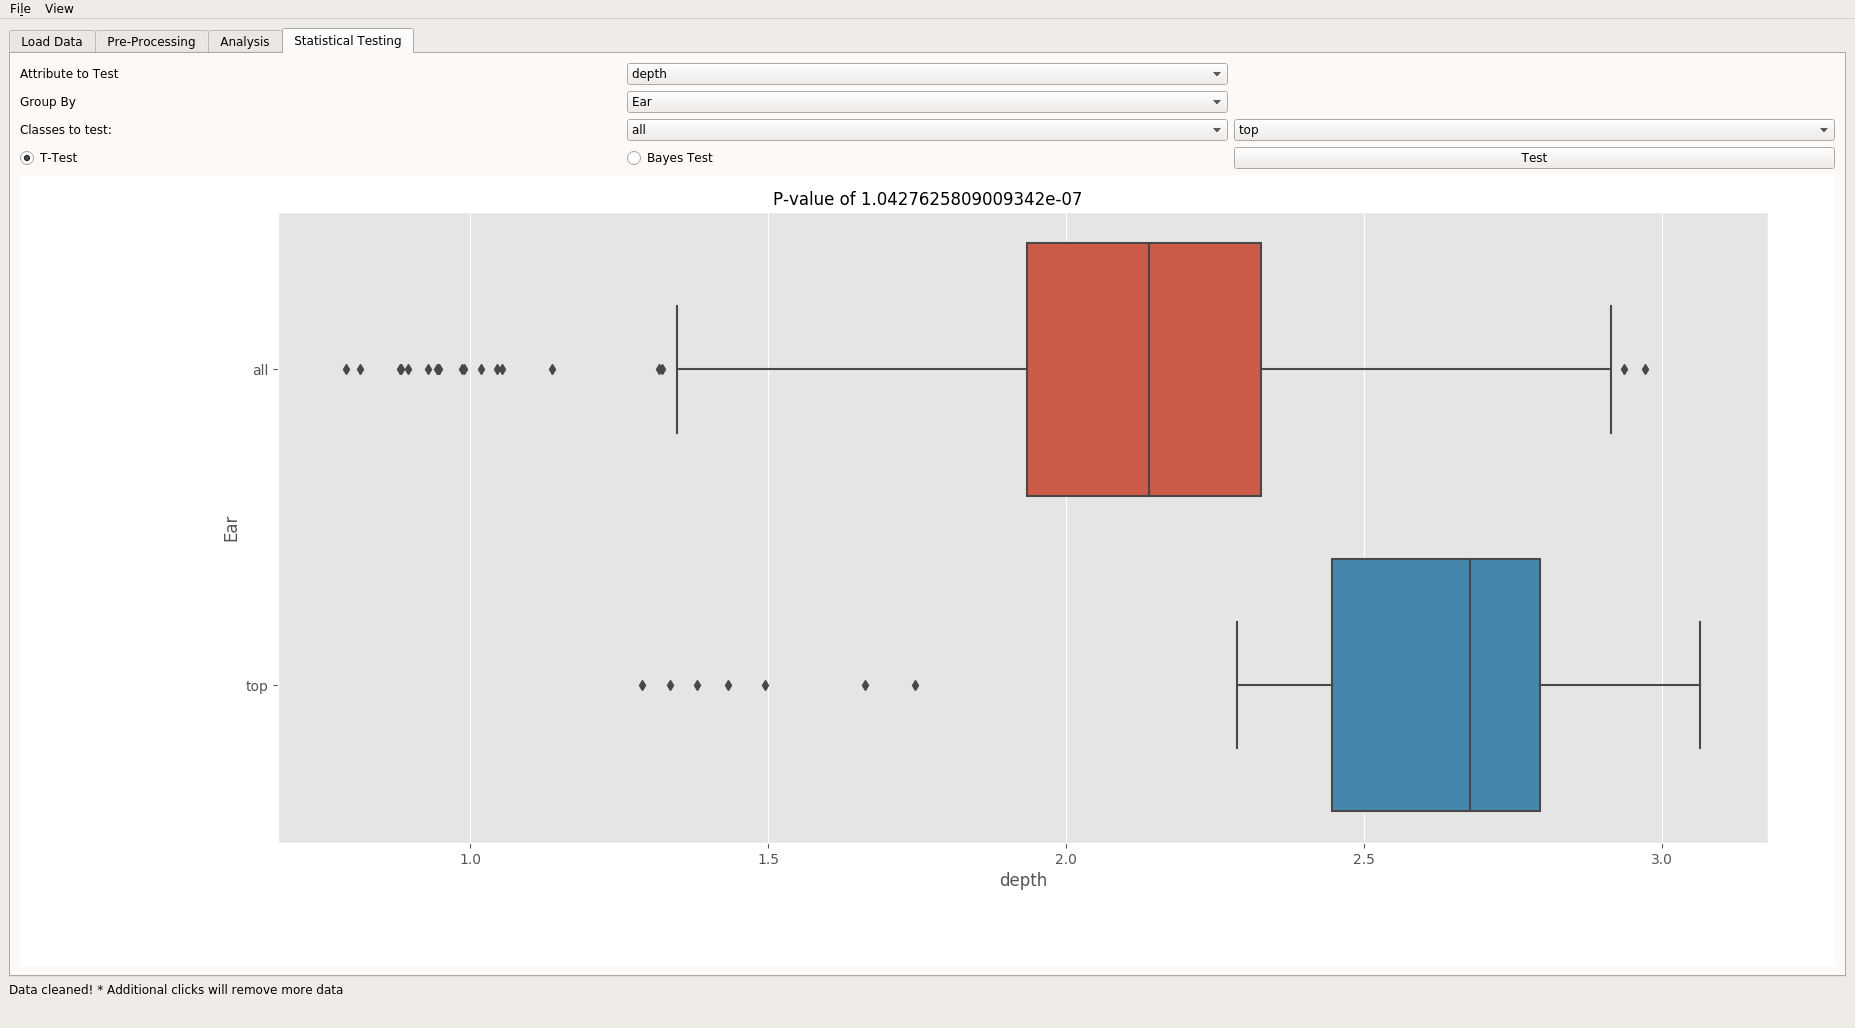
\includegraphics[width=.9\linewidth]{./images/Screenshots/hypothesis_ttest_g1_att_1.png}
\end{center}\\
\hline
28 & \color{ForestGreen}Passed & analysis.py:: box\_rb\_2 & N/A\\
\hline
29 & \color{ForestGreen}Passed & analysis.py:: hist\_groupby\_1\_rb\_2 & N/A\\
\hline
30 & \color{ForestGreen}Passed & analysis.py:: hist\_rb\_2 & N/A\\
\hline
31 & \color{ForestGreen}Passed & analysis.py:: loads & N/A\\
\hline
32 & \color{ForestGreen}Passed & hypothesis\_tests.py:: bayesg1\_att\_2 & N/A\\
\hline
33 & \color{ForestGreen}Passed & hypothesis\_tests.py:: bayesg2\_att\_1 & N/A\\
\hline
34 & \color{ForestGreen}Passed & hypothesis\_tests.py:: bayesg2\_att\_2 & N/A\\
\hline
35 & \color{ForestGreen}Passed & hypothesis\_tests.py:: tg1\_att\_2 & N/A\\
\hline
36 & \color{ForestGreen}Passed & hypothesis\_tests.py:: tg2\_att\_1 & N/A\\
\hline
37 & \color{ForestGreen}Passed & hypothesis\_tests.py:: tg2\_att\_2 & N/A\\
\hline
38 & \color{ForestGreen}Passed & hypothesis\_tests.py:: loads & N/A\\
\hline
39 & \color{ForestGreen}Passed & GUI.py:: startup & N/A\\
\hline
40 & \color{ForestGreen}Passed & load\_data.py:: load\_data\_with\_rachis & N/A\\
\hline
41 & \color{ForestGreen}Passed & load\_data.py:: load\_data\_without\_rachis & N/A\\
\hline
42 & \color{ForestGreen}Passed & preprocessing.py:: clean\_data\_remove\_large & N/A\\
\hline
43 & \color{ForestGreen}Passed & preprocessing.py:: clean\_data\_remove\_none & N/A\\
\hline
44 & \color{ForestGreen}Passed & preprocessing.py:: clean\_data\_remove\_small & N/A\\
\hline
45 & \color{ForestGreen}Passed & preprocessing.py:: clean\_data\_remove \_small\_and\_large & N/A\\
\hline
46 & \color{ForestGreen}Passed & preprocessing.py:: load\_additional\_data & N/A\\
\hline
47 & \color{ForestGreen}Passed & preprocessing.py:: load\_additional\_data \_expected\_fail & N/A\\
\hline
\end{longtable}

\subsection{Acceptance Testing}
\label{sec:orgb8dba66}
These unit tests, alongside user tests have been used to meet the outlined functional requirements; specific tests are shown in table:\ref{tab:orgd1ce2c6} to match them to the associated functional requirement.

\begin{longtable}{|l|l|p{14cm}|}
\caption{\label{tab:orgd1ce2c6}
Functional requirements and Unit tests}
\\
\hline
\textbf{F.R.} & \textbf{U.T.} & \textbf{How is the F.R. met?}\\
\hline
\endfirsthead
\multicolumn{3}{l}{Continued from previous page} \\
\hline

\textbf{F.R.} & \textbf{U.T.} & \textbf{How is the F.R. met?} \\

\hline
\endhead
\hline\multicolumn{3}{r}{Continued on next page} \\
\endfoot
\endlastfoot
\hline
0 & n/a & An OOP interface is provided by the \emph{ct\_data} object\\
\hline
1 & 3,4,5 & Loading of data is tested multiple times specifically through unit tests\\
\hline
2 & 4,5 & Unit tests carry out saving loaded data into appropriate formats, in particular python \emph{pandas} tables and CSV files, this was also user tested\\
\hline
3 & 7,8,9,10 & All the functions in the \emph{data\_transforms.py} library are unit tested automatically on test data of known output\\
\hline
4 & 26,27,32-38 & Hypothesis testing was tested with known data 8+ times in automated unit testing for both CT GUI Application and the CT Analysis Library group of tests , testers also used these functions\\
\hline
5 & 6,7 & Loading of spikes was tested both for data which was known to exist and could be successfully done, and for data which was know to throw errors\\
\hline
6 & 1,2,7,42-46 & Finding and removing erroneous data was unit tested by having a combination of parameters tested for both the GUI and the Analysis Library\\
\hline
7 & 3-6,40,41 & Matching of pre-existing experiment information to the extracted data was tested for bad inputs through unit testing, users tested this too and reported no unexpected results\\
\hline
8 & 11-17,28-38 & Plotting of data automatically, inferring of axis, titles and measurements was tested, with images automatically recorded by unit tests.\\
\hline
9 & 0,1,2,3 & Unit testing checked if given data could easily be separated and divided into subsections, this was specifically tested and tested by proxy in other tests when hypothesis testing was performed\\
\hline
10 & 21,26 39,40,42 & Multiple tests are taken to check that the GUI loads as expected, planning sessions and user feedback was also used to meet this particular functional requirement\\
\hline
11 & 40,42 & Data is loaded through GUI elements with little prior knowledge of the software in order to have data processed, this was unit tested and user feedback was used to make more accessible\\
\hline
12 & 21-27 & Testing of \emph{Matplotlib} and \emph{Seaborn} interfacing with, and integrating with the CT Analysing GUI.\\
\hline
13 & 43-47 & Loading of experiment data is pivotal for most functionality of the GUI, it is tested multiple times in an isolated formatted, as well as by other future functions which require it\\
\hline
14 & n/a & The entire software is wrapped in an MVC model, this cannot be tested but the functional requirement has been met\\
\hline
15 & 21-47 & All of the unit tests for the CT Analysing GUI depend on the CT Analysing Library, it is reasonable that the integration is well tested, by product of all other tests\\
\hline
16 & 21-27 & Several tests, those shown in table:\ref{tab:org26e75de} are specifically recorded visually and presented as images in order to automatically unit test that visual data is intact\\
\hline
17 & 21-27 & By using automatic image capturing of unit testing in progress, visual checking can be carried out and confirmed that data is visually what is expected and to a high standard\\
\hline
18 & 26,27, 32-28 & With multiple known outputs, several different groupings and combinations the hypothesis tests were unit tested and this functional requirement is known to be acceptably implemented\\
\hline
\end{longtable}

\chapter{Methods and Solutions}
\label{sec:org2cfe658}
This chapter will discuss and expand upon the software implementations which were carried out in the course of this project, with particular focus on novel and non-trivial elements.

Where appropriate code segments snipp

\section{Data Pipeline}
\label{sec:orgdd2c130}

\begin{figure}[htbp]
\centering
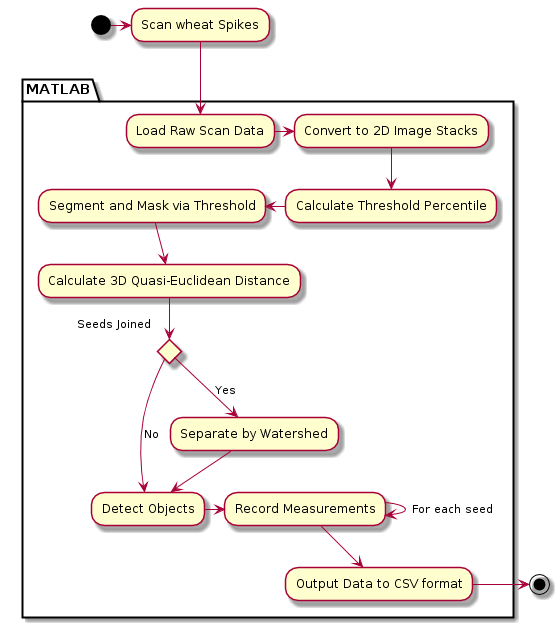
\includegraphics[width=13cm]{./images/matlab.png}
\caption{\label{fig:org1047412}
Image Processing Pipeline}
\end{figure}

\section{Image Analysis Methods}
\label{sec:orgec3314a}
\subsection{New Watershed Algorithm}
\label{sec:org754a052}

In order to solve the problem of misidentified and joint seeds, from the primitive collection,
a  \emph{quasi-euclidean} distance transform was implemented into the analysis pipeline (figure:). This provided much better results than the previous
\emph{chessboard} transform which had been successful on more uniform data in previous studies \cite{Hughes2017}.

\subsubsection{Quasi-Euclidean algorithm}
\label{sec:org44df04f}

This algorithm measures the total euclidean distance along a set of horizontal, vertical and diagonal
line segments \cite{Pfaltz1966}.

\begin{equation}
\label{eq:org68149db}
\left | x_1 - x_2 \right | + (\sqrt{2}-1), \left | x_1 - x_2 \right | >\left | y_1 - y_2 \right | (\sqrt{2}-1) \left | x_1 - x_2 \right | ,\textup{otherwise}
\end{equation}



In order to apply this to a 3D space Kleinberg's method is used  \cite{Kleinberg1997}. This allows for nearest neighbour pixels to be sorted by \$k\$-dimensional trees
and enabling fast distance transforms via Rosenfeld and Pfaltz's \emph{quasi-euclidean} method stated in equation:\ref{eq:org68149db}.
\subsubsection{Effect of Enhanced Watershed algorithm}
\label{sec:org152f02a}
\begin{center}
\begin{figure}[htbp]
\centering
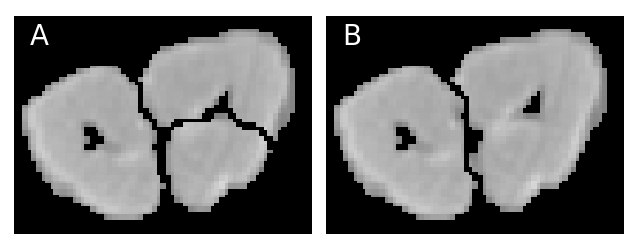
\includegraphics[width=10cm]{./images/chess_quasi.png}
\caption{\label{fig:orgebbbb53}
\emph{A} showing the chessboard method, \emph{B} improved quasi-euclidean method}
\end{figure}
\end{center}

\subsection{Extracted Grains}
\label{sec:org5e5fc3b}

\begin{figure}[htbp]
\centering
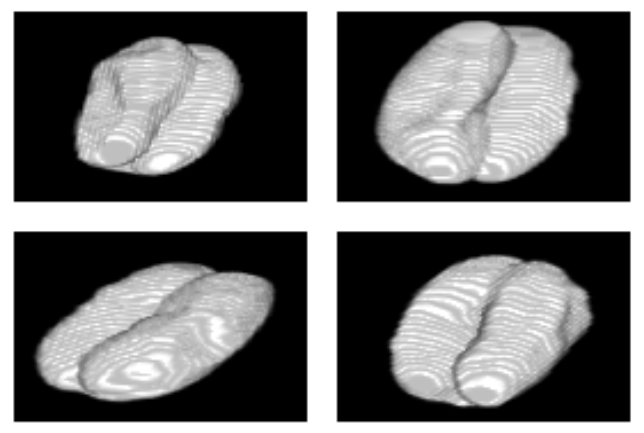
\includegraphics[width=13cm]{./images/ctgrains.png}
\caption{\label{fig:org24df965}
Individual Wheat grains, rendered in 3D}
\end{figure}

\section{CT Analysing Library Methods}
\label{sec:org48de281}
\subsection{Spike Rejoining}
\label{sec:org2222086}
\subsection{Data Aggregating}
\label{sec:org996df8a}
\subsection{Loading Data}
\label{sec:org60b831b}
\subsection{Cleaning and Removing Erroneous Data}
\label{sec:orge5cecde}
\subsection{Data Transformations}
\label{sec:org5767c3b}
\subsection{T-Tests}
\label{sec:org93ea550}
\subsection{Bayesian Hypothesis Testing}
\label{sec:org90d7eb7}
\subsection{Plotting Functions}
\label{sec:org411c673}
\subsection{Adding Spike Experiment Information}
\label{sec:orgc9ff9d0}
\begin{listing}[htbp]
\begin{minted}[]{python}
def get_spike_info(grain_df, excel_file, join_column='Folder#'):

    # Make a copy as we don't want to change the original
    df = grain_df.copy(deep=True)

    # Grab the linking excel file
    info = pd.read_excel(excel_file,
                         index_col='Folder#')

    # These are the features to grab
    features = ['Hulled/Naked', 'Common name', 'Genome', 'Ploidy',
                'Wild/Domesticated', 'Sample name', 'Sub type', 'Ear']

    # Lambda to look up the feature in excel spreadsheet
    def look_up(x, y): return info.loc[x['folderid']][y]

    # Lambda form a series (data row) and apply it to dataframe
    def gather_data(x): return pd.Series([look_up(x, y) for y in features])

    df[features] = df.apply(gather_data, axis=1)

    # Return the copy
    return df
\end{minted}
\caption{\label{orge75c7bc}
Spike Information Joining Algorithm}
\end{listing}

\section{CT GUI Application Methods}
\label{sec:org832ffbb}
\subsection{Integration with CT Analysis Library}
\label{sec:org697814d}
\subsection{QT GUI Loading}
\label{sec:org498af30}
\subsection{Connecting Signals from GUI to Function Calls}
\label{sec:org9800203}
\subsection{Plot Window Rendering}
\label{sec:orgb14be76}
\subsection{Creating GUI Elements When Required}
\label{sec:org7cb91cb}
\subsection{Dynamically Generating Plots}
\label{sec:orgeb36a01}
\section{Data Analysis Methods}
\label{sec:org9061736}

\begin{figure}[htbp]
\centering
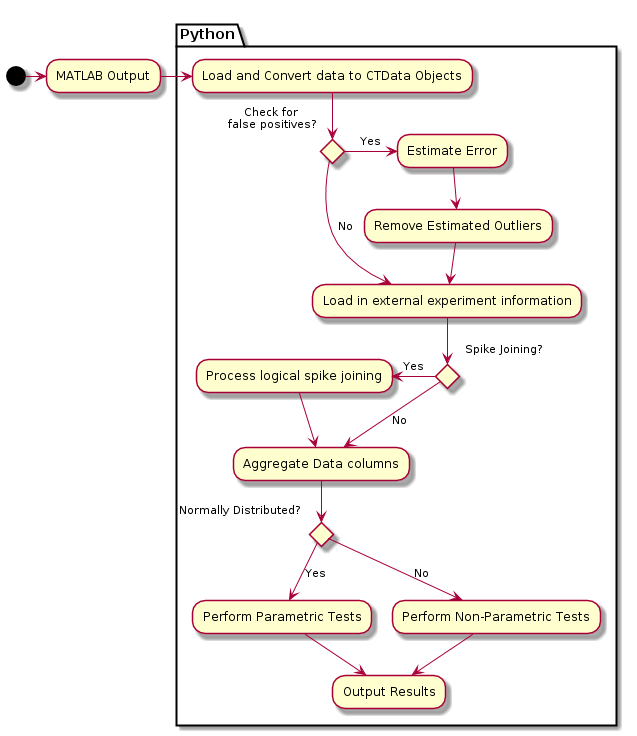
\includegraphics[width=13cm]{./images/pipeline.png}
\caption{\label{fig:org390f702}
How data is integrated with the CT Analysing Library}
\end{figure}

\chapter{Results}
\label{sec:org64e4c21}
\chapter{Discussion}
\label{sec:org26cda71}
\section{Similar Research}
\label{sec:org762f751}
\section{Alternate Solutions}
\label{sec:orgc09f5c9}
\chapter{Critical Evaluation}
\label{sec:org0b39b54}
\section{Organisational Methods}
\label{sec:org53a8ea8}
\section{Relevance to Degree}
\label{sec:org93619ba}
\section{Time Management}
\label{sec:orga31ef08}
\section{Collaborative Work}
\label{sec:org53f7b6e}
\section{Other Issues}
\label{sec:org01d2572}
\chapter{Appendix}
\label{sec:org5f93600}
\section{\emph{Software Packages Used}}
\label{sec:orgcbfbbb8}

\subsection{Libraries}
\label{sec:org222b6c6}
\begin{table}[htbp]
\caption{\label{tab:orgd79dfdb}
Software libraries used}
\centering
\begin{tabularx}{\textwidth}{|X|X|X|}
\hline
Seaborn & Scipy & Sklearn\\
\hline
MATLAB Image Processing Toolbox & Numpy & Matplotlib\\
\hline
Statsmodels & Pymc3 & Xlrd\\
\hline
PyQt5 & gcc & Pip\\
\hline
\end{tabularx}
\end{table}

\subsection{Tools}
\label{sec:org54393b1}
\begin{table}[htbp]
\caption{\label{tab:orgb466f0b}
Software tools used}
\centering
\begin{tabularx}{\textwidth}{|X|X|X|}
\hline
MATLAB & Python Debugger (PDB) & IPython\\
\hline
Emacs & git & org-mode\\
\hline
Tomviz & ImageJ & PlantUML\\
\hline
\end{tabularx}
\end{table}

\clearpage
\section{\emph{Glossary}}
\label{sec:orgc256d4c}
\begin{table}[htbp]
\caption{\label{tab:orgcf883cd}
Dictionary for Terms and acronyms}
\centering
\begin{tabularx}{\textwidth}{|l|X|}
\hline
\textbf{Term} & \textbf{Definition}\\
\hline
\textmu{}-CT & Micro Computed Tomography\\
\hline
Genotype & A genetically distinct individual or group\\
\hline
Phenotype & A physical/measurable trait\\
\hline
Alleles & A variant of a gene\\
\hline
Genus & Classification ranking, below the \emph{family} grouping\\
\hline
Genome & The complete genetic make up of an organism, which defines its individuality\\
\hline
Morphometric & The shape and form of an organism\\
\hline
GUI & Graphical User Interface\\
\hline
PCA & Principal Component Analysis\\
\hline
Spike & A singular stalk of wheat\\
\hline
Spikelet & A group of seeds all forming from the same node in a spike\\
\hline
MVC & Model View Controller - A design pattern for GUIs\\
\hline
OOP & Object Orientated Programming\\
\hline
\end{tabularx}
\end{table}

\clearpage
\section{Wheat Varieties}
\label{sec:org22dcedb}
\begin{table}[htbp]
\caption{\label{tab:org96d26e3}
Wheat used in this work and their common names}
\centering
\begin{tabularx}{\textwidth}{|X|X|}
\hline
\textbf{Species name} & \textbf{Common name}\\
\hline
\emph{Triticum monococcum} & Einkorn Domesticate\\
\hline
\emph{Triticum boeticum} & Einkorn Wild\\
\hline
\emph{Aegilops tauschii} & n/a\\
\hline
\emph{Triticum durum} & Pasta Wheat\\
\hline
\emph{Triticum dicoccoides} & Einkorn Domesticate\\
\hline
\emph{Triticum dicoccum} & Einkorn Wild\\
\hline
\emph{Triticum ispahanicum} & n/a\\
\hline
\emph{Triticum timopheevii} & n/a\\
\hline
\emph{Triticum spelta} & Spelt\\
\hline
\emph{Triticum aestivum} & Bread Wheat\\
\hline
\emph{Triticum compactum} & Club Wheat\\
\hline
\end{tabularx}
\end{table}



\clearpage
\section{\emph{Code Segments and Examples}}
\label{sec:org0590615}
\subsection{MATLAB Watershedding}
\label{sec:orgf6fc972}

\begin{listing}[htbp]
\begin{minted}[]{octave}
function [W] = watershedSplit3D(A)
  % Takes image stack A and splits it into stack W
  % Convert to BW
  bw = logical(A);
  % Create variable for opening and closing
  se = strel('disk', 5);
  % Minimise object missshapen-ness
  bw = imerode(bw, se);
  bw = imdilate(bw, se);
  % Fill in any left over holes
  bw = imfill(bw,4,'holes');
  % Use chessboard for distance calculation for more refined splitting
  chessboard = -bwdist(~bw, 'quasi-euclidean');
  % Modify the intensity of our bwdist to produce chessboard2
  mask = imextendedmin(chessboard, 2);
  chessboard2 = imimposemin(chessboard, mask);
  % Calculate watershed based on the modified chessboard
  Ld2 = watershed(chessboard2);
  % Take original image and add on the lines calculated for splitting
  W = A;
  W(Ld2 == 0) = 0;
end
\end{minted}
\caption{\label{org71c0a2b}
MATLAB Watershedding function}
\end{listing}

\clearpage
\subsection{Custom Documentation Generator}
\label{sec:org9a9a60b}
\begin{listing}[htbp]
\begin{minted}[]{common-lisp}
(defun populate-org-buffer (buffer filename root)
  (goto-char (point-min))
  (let ((to-insert (concat "* " (replace-regexp-in-string root "" filename) "\n") ))
    (while (re-search-forward
            (rx (group (or "def" "class"))
                space
                (group (+ (not (any "()"))))
                (? "(" (* nonl) "):" (+ "\n") (+ space)
                   (= 3 "\"")
                   (group (+? anything))
                   (= 3 "\"")))
            nil 'noerror)
      (setq to-insert
            (concat
             to-insert
             (if (string= "class" (match-string 1))
                 "** "
               "*** ")
             (match-string 2)
             "\n"
             (and (match-string 3)
                  (concat (match-string 3) "\n")))))helm-semantic-or-imenu
    (with-current-buffer buffer
      (insert to-insert))))
(defun org-documentation-from-dir (&optional dir)
  (interactive)
  (let* ((dir  (or dir (read-directory-name "Choose base directory: ")))
         (files (directory-files-recursively dir "\py$"))
         (doc-buf (get-buffer-create "org-docs")))
    (dolist (file files)
      (with-temp-buffer
        (insert-file-contents file)
        (populate-org-buffer doc-buf file dir)))
    (with-current-buffer doc-buf
      (org-mode))))
\end{minted}
\caption{\label{org1db3016}
Custom lisp code for generating easy to read documentation}
\end{listing}

\clearpage
\subsection{Self-Documenting Code Example}
\label{sec:org4cd5ae7}
\begin{listing}[htbp]
\begin{minted}[]{python}
def get_spike_info(self, excel_file, join_column='Folder#'):
    """
    This function should do something akin to adding additional
    information to the data frame

    @note there is some confusion in the NPPC about whether to use
    folder name or file name as the unique id when this is made into
    end-user software, a toggle should be added to allow this

    @param excel_file a file to attach and read data from
    @param join_column if the column for joining data is
    different then it should be stated
    """
    try:
        # Grab the linking excel file
        info = pd.read_excel(excel_file,
                             index_col='Folder#')

        features = list(info.columns)
        # Lambda to look up the feature in excel spreadsheet
        def look_up(x, y): return info.loc[x['folderid']][y]

        # Lambda form a series (data row) and apply it to dataframe
        def gather_data(x): return pd.Series(
            [look_up(x, y) for y in features])

        self.df[features] = self.df.apply(gather_data, axis=1)
    except KeyError as e:
        print('Error matching data')
        print(e)
        raise NoDataFoundException
    except AttributeError as e:
        print(e)
        raise NoDataFoundException

\end{minted}
\caption{\label{org52bea07}
Example of code documentation and readability from \emph{data\_transforms.py}}
\end{listing}
\clearpage
\subsection{Setup.py}
\label{sec:orgf3b9a30}
\begin{listing}[htbp]
\begin{minted}[]{python}
from setuptools import setup
setup(name='CT_Analysing_Library',
      version='0.2',
      description='Library used for CT grain analysis at the NPPC',
      url='https://github.com/SirSharpest/CT_Analysing_Library',
      author='Nathan Hughes',
      author_email='nathan1hughes@gmail.com',
      license='MIT',
      packages=['ct_analysing_library'],
      install_requires=['pandas',
                        'numpy',
                        'matplotlib',
                        'seaborn',
                        'scipy',
                        'sklearn',
                        'statsmodels',
                        'pymc3',
                        'xlrd'],
      zip_safe=True)
\end{minted}
\caption{\label{org6334f9d}
The \emph{setup.py} configuration for the CT Analyser Library}
\end{listing}

\clearpage
\bibliography{library}
\bibliographystyle{IEEEannotU}
\end{document}
